%% This is the ctufit-thesis example file. It is used to produce theses
%% for submission to Czech Technical University, Faculty of Information Technology.
%%
%% Get the newest version from
%% https://gitlab.fit.cvut.cz/theses-templates/FITthesis-LaTeX
%%
%%
%% Copyright 2021, Eliska Sestakova and Ondrej Guth
%%
%% This work may be distributed and/or modified under the
%% conditions of the LaTeX Project Public Licenese, either version 1.3
%% of this license or (at your option) any later version.
%% The latest version of this license is in
%%  https://www.latex-project.org/lppl.txt
%% and version 1.3 or later is part of all distributions of LaTeX
%% version 2005/12/01 or later.
%%
%% This work has the LPPL maintenance status `maintained'.
%%
%% The current maintainer of this work is Ondrej Guth.
%% Contact ondrej.guth@fit.cvut.cz for bug reports.
%% Alternatively, submit bug reports into the tracker at
%% https://gitlab.fit.cvut.cz/theses-templates/FITthesis-LaTeX/issues
%%
%%

%%%%%%%%%%%%%%%%%%%%%%%%%%%%%%%%%%%%%%%%%
% CLASS OPTIONS
% language: czech/english/slovak
% thesis type: bachelor/master/dissertation
% colour: bw for black&white OR no option for default colour scheme
%%%%%%%%%%%%%%%%%%%%%%%%%%%%%%%%%%%%%%%%%
\documentclass[czech,bachelor,unicode]{ctufit-thesis}

%%%%%%%%%%%%%%%%%%%%%%%%%%%%%%%%%%
% FILL IN THIS INFORMATION
%%%%%%%%%%%%%%%%%%%%%%%%%%%%%%%%%%
\ctufittitle{Emulátor konzole Nintendo Entertainment System} % replace with the title of your thesis
\ctufitauthorfull{Ondřej Golasowski} % replace wit¨h your full name (first name(s) and then family name(s) / surname(s)) including academic degrees
\ctufitauthorsurnames{Golasowski} % replace with your surname(s) / family name(s)
\ctufitauthorgivennames{Ondřej} % replace with your first name(s) / given name(s)
\ctufitsupervisor{Ing.\,Stanislav Jeřábek} % replace with name of your supervisor/advisor (include academic degrees)
\ctufitdepartment{Katedra číslicového návrhu } % replace with the department of your defence
\ctufityear{2023} % replace with the year of your defence
\ctufitdeclarationplace{Praze} % replace with the place where you sign the declaration
\ctufitdeclarationdate{\today} % replace with the date of signature of the declaration
\ctufitabstractCZE{Fill in abstract of this thesis in Czech language. Class aptent taciti sociosqu ad litora torquent per conubia nostra, per inceptos hymenaeos. Cras pede libero, dapibus nec, pretium sit amet, tempor quis. Sed vel lectus. Donec odio tempus molestie, porttitor ut, iaculis quis, sem. Suspendisse sagittis ultrices augue.}
\ctufitabstractENG{Fill in abstract of this thesis in English language. Class aptent taciti sociosqu ad litora torquent per conubia nostra, per inceptos hymenaeos. Cras pede libero, dapibus nec, pretium sit amet, tempor quis. Sed vel lectus. Donec odio tempus molestie, porttitor ut, iaculis quis, sem. Suspendisse sagittis ultrices augue.}
\ctufitkeywordsCZE{enter, commma, separated, list, of, keywords, in, CZECH}
\ctufitkeywordsENG{enter, commma, separated, list, of, keywords, in, ENGLISH}
%%%%%%%%%%%%%%%%%%%%%%%%%%%%%%%%%%
% END FILL IN
%%%%%%%%%%%%%%%%%%%%%%%%%%%%%%%%%%

%%%%%%%%%%%%%%%%%%%%%%%%%%%%%%%%%%
% CUSTOMIZATION of this template
% Skip this part or alter it if you know what you are doing.
%%%%%%%%%%%%%%%%%%%%%%%%%%%%%%%%%%
\RequirePackage{iftex}[2020/03/06]
\iftutex % XeLaTeX and LuaLaTeX
    \RequirePackage{ellipsis}[2020/05/22] %ellipsis workaround for XeLaTeX
\else
    \RequirePackage[utf8]{inputenc}[2018/08/11] %this file encoding
    \RequirePackage{lmodern}[2009/10/30] % vector flavor of Computer Modern font
\fi

% hyperlinks
\RequirePackage[pdfpagelayout=TwoPageRight,colorlinks=false,allcolors=decoration,pdfborder={0 0 0.1}]{hyperref}[2020-05-15]

% uncomment the following to hide all hyperlinks
% \RequirePackage[pdfpagelayout=TwoPageRight,hidelinks]{hyperref}[2020-05-15]

\RequirePackage{pdfpages}[2020/01/28]

\setcounter{secnumdepth}{4} % numbering sections; 4: subsubsection

\definecolor{bfcommon}{RGB}{250, 159, 66}
\definecolor{bfcommonlight}{RGB}{253, 214, 176}
\definecolor{bfaux}{RGB}{71, 188, 255}
\definecolor{bfauxlight}{RGB}{194, 233, 255}

\definecolor{fcaction}{RGB}{253, 214, 176}
\definecolor{fcbranch}{RGB}{194, 233, 255}
\definecolor{fcstart}{RGB}{250, 159, 66}

\definecolor{mastercomponent}{RGB}{71, 188, 255}
\definecolor{slavecomponent}{RGB}{250, 159, 66}
\definecolor{interface}{RGB}{253, 214, 176}

%%%%%%%%%%%%%%%%%%%%%%%%%%%%%%%%%%
% CUSTOMIZATION of this template END
%%%%%%%%%%%%%%%%%%%%%%%%%%%%%%%%%%


%%%%%%%%%%%%%%%%%%%%%%
% DEMO CONTENTS SETTINGS
% You may choose to modify this part.
%%%%%%%%%%%%%%%%%%%%%%
\usepackage{dirtree}
\usepackage{lipsum,tikz}
\usetikzlibrary{positioning, shapes.geometric, calc, arrows, decorations.pathreplacing}
\usepackage{csquotes}
\usepackage[style=iso-numeric]{biblatex}
\addbibresource{text/bib-database.bib}
%\usepackage{listings} % typesetting of sources
\usepackage{minted} % typesetting of sources
\counterwithin{listing}{chapter}
\usepackage{epigraph}
\usepackage{tikz-timing}
\usetikztiminglibrary[rising arrows]{clockarrows}
\usepackage{xparse}
\usepackage{bytefield}
\usepackage{tabularray}

%theorems, definitions, etc.
\theoremstyle{plain}
\newtheorem{theorem}{Věta}
\newtheorem{lemma}[theorem]{Tvrzení}
\newtheorem{corollary}[theorem]{Důsledek}
\newtheorem{proposition}[theorem]{Návrh}
\newtheorem{definition}[theorem]{Definice}
\theoremstyle{definition}
\newtheorem{example}[theorem]{Příklad}
\theoremstyle{remark}
\newtheorem{note}[theorem]{Poznámka}
\newtheorem*{note*}{Poznámka}
\newtheorem{remark}[theorem]{Pozorování}
\newtheorem*{remark*}{Pozorování}
\numberwithin{theorem}{chapter}
%theorems, definitions, etc. END
%%%%%%%%%%%%%%%%%%%%%%
% DEMO CONTENTS SETTINGS END
%%%%%%%%%%%%%%%%%%%%%%

%%%%%%%%%%%%%%%%%%%%%%
% CUSTOM XPARSE COMMANDS
%%%%%%%%%%%%%%%%%%%%%%
% Reference a signal.
%
% Usage:
%
%     \signal[3::0]{C/BE}    ->   C/BE[3::0]
%     \signal*{AD}           ->   AD#
%     \signal*[3::0]{C/BE}   ->   C/BE[3::0]#
%
% By Nathan Typanski from: https://nathantypanski.com/blog/2014-10-29-tikz-timing.html#fn1\textbf
\NewDocumentCommand{\signal}{som}{\texttt{%
		#3%
		\IfValueTF{#2}{[#2]}{}%
		\IfBooleanTF{#1}{\#}{}%
}}
%%%%%%%%%%%%%%%%%%%%%%
% XPARSE COMMANDS END
%%%%%%%%%%%%%%%%%%%%%%

\begin{document} 
\frontmatter\frontmatterinit % do not remove these two commands

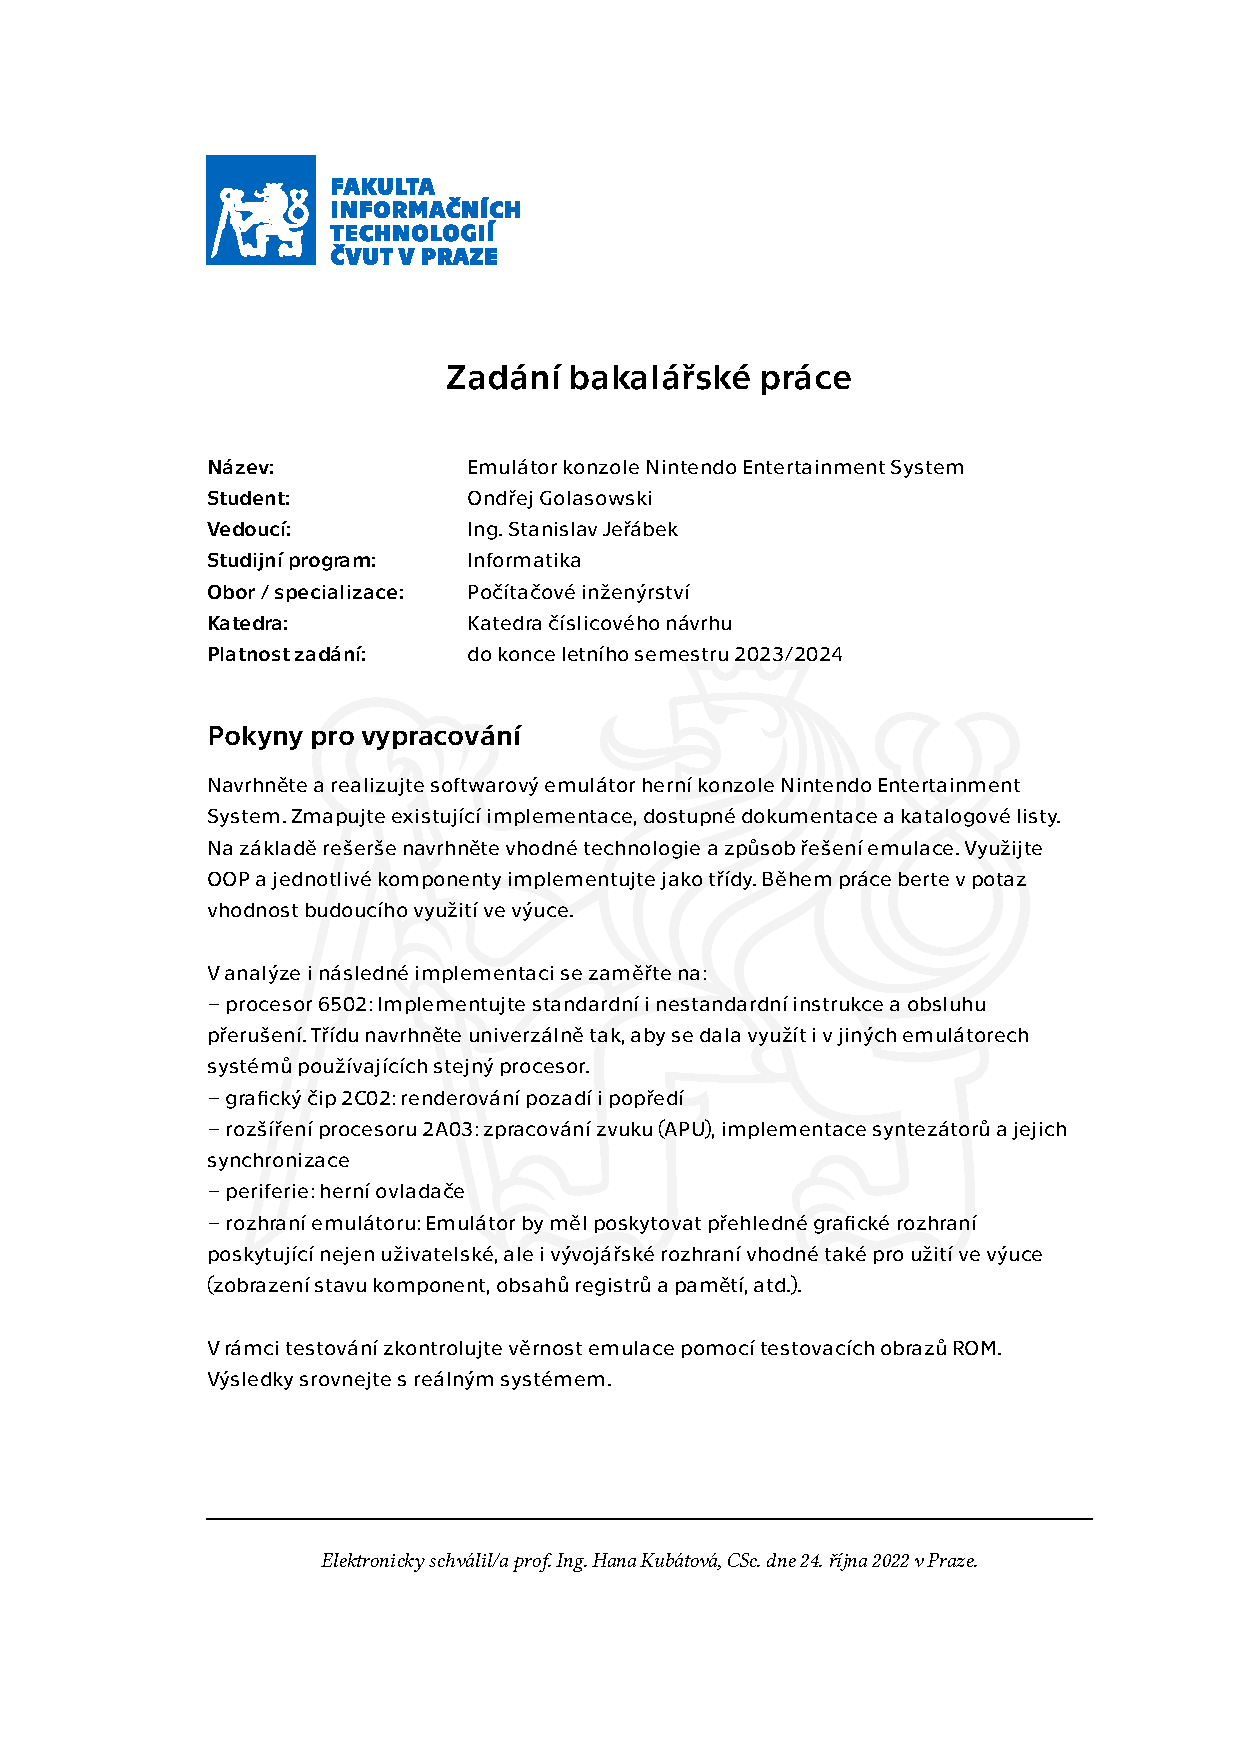
\includepdf[pages={1-}]{assignment-include.pdf} % replace that file with your thesis assignment provided by study office

\thispagestyle{empty}\cleardoublepage\maketitle % do not remove these three commands

\imprintpage % do not remove this command

\tableofcontents % do not remove this command
%%%%%%%%%%%%%%%%%%%%%%
% list of other contents: figures, tables, code listings, algorithms, etc.
% add/remove commands accordingly
%%%%%%%%%%%%%%%%%%%%%%
\listoffigures % list of figures
\begingroup
\let\clearpage\relax
\listoftables % list of tables
%\lstlistoflistings % list of source code listings generated by the listings package
\listoflistings % list of source code listings generated by the minted package
\endgroup
%%%%%%%%%%%%%%%%%%%%%%
% list of other contents END
%%%%%%%%%%%%%%%%%%%%%%

%%%%%%%%%%%%%%%%%%%
% ACKNOWLEDGMENT
% FILL IN / MODIFY
% This is a place to thank people for helping you. It is common to thank your supervisor.
%%%%%%%%%%%%%%%%%%%
\begin{acknowledgmentpage}
	Chtěl bych poděkovat především komunitě nesdev.org, která seskupila dokumentaci k celému emulovanému systému, poskytla mnoho užitečných faktů, pozorování a testů. Děkuji také vedoucímu práce Ing.\,Stanislavovi~Jeřábkovi za věcné podněty při vypracovávání analytické, implementační i textové části bakalářské práce.
\end{acknowledgmentpage} 
%%%%%%%%%%%%%%%%%%%
% ACKNOWLEDGMENT END
%%%%%%%%%%%%%%%%%%%


%%%%%%%%%%%%%%%%%%%
% DECLARATION
% FILL IN / MODIFY
%%%%%%%%%%%%%%%%%%%
% INSTRUCTIONS
% ENG: choose one of approved texts of the declaration. DO NOT CREATE YOUR OWN. Find the approved texts at https://courses.fit.cvut.cz/SFE/download/index.html#_documents (document Declaration for FT in English)
% CZE/SLO: Vyberte jedno z fakultou schvalenych prohlaseni. NEVKLADEJTE VLASTNI TEXT. Schvalena prohlaseni najdete zde: https://courses.fit.cvut.cz/SZZ/dokumenty/index.html#_dokumenty (prohlášení do ZP)
\begin{declarationpage}
Prohlašuji, že jsem předloženou práci vypracoval samostatně a že jsem uvedl veškeré
použité informační zdroje v~souladu s Metodickým pokynem o~dodržování etických
principů při přípravě vysokoškolských závěrečných prací.

Beru na vědomí, že se na moji práci vztahují práva a povinnosti vyplývající ze zákona
č.~121/2000~Sb., autorského zákona, ve znění pozdějších předpisů. V souladu s~ust.
§~2373~odst.~2 zákona č.~89/2012~Sb., občanský zákoník, ve znění pozdějších předpisů,
tímto uděluji nevýhradní oprávnění (licenci) k~užití této mojí práce, a to včetně všech
počítačových programů, jež jsou její součástí či přílohou a veškeré jejich
dokumentace (dále souhrnně jen \uv{Dílo}), a to všem osobám, které si přejí Dílo užít.
Tyto osoby jsou oprávněny Dílo užít jakýmkoli způsobem, který nesnižuje hodnotu
Díla, avšak pouze k~nevýdělečným účelům. Toto oprávnění je časově, teritoriálně
i~množstevně neomezené.
\end{declarationpage}
%%%%%%%%%%%%%%%%%%%
% DECLARATION END
%%%%%%%%%%%%%%%%%%%

\printabstractpage % do not remove this command

%%%%%%%%%%%%%%%%%%%
% SUMMARY
% FILL IN / MODIFY
% OR REMOVE ENTIRELY (upon agreement with your supervisor)
% (appropriate to remove in most theses)
%%%%%%%%%%%%%%%%%%%
\begin{summarypage}
\section*{Summary section}

\lipsum[1][1-8]

\section*{Summary section}

\lipsum[2][1-6]

\section*{Summary section}

\lipsum[3]

\section*{Summary section}

\lipsum[2]

\section*{Summary section}

\lipsum[1][1-8] Lorem lorem lorem.
\end{summarypage}
%%%%%%%%%%%%%%%%%%%
% SUMMARY END
%%%%%%%%%%%%%%%%%%%

%%%%%%%%%%%%%%%%%%%
% ABBREVIATIONS
% FILL IN / MODIFY
% OR REMOVE ENTIRELY
% List the abbreviations in lexicography order.
%%%%%%%%%%%%%%%%%%%
\chapter{Seznam zkratek}
\begin{tabular}{rl}
	ASIC & Application Specific Integrated Circuit \\
	PLA & Programmable Logic Array \\
	A & akumulátor \\
	S & stack pointer \\
	PC & program counter \\
OZ & operační znak \\
ADL & address low \\
ADH & address high \\
NMI & non-maskable interrupt\\
IRQ & interrupt request\\
OOP & objektově orientované programování \\
VRAM & Video RAM\\
NTSC & National Television System Committee\\
I/O & input/output \\
PAL &  Phase Alternating Line\\
CPU & central processing unit\\
ROM & read only memory\\
RAM & random access memory\\
OAM & object attribute memory\\
JSA & jazyk symbolických adres\\
NES & Nintendo Entertainment System\\
FC & Family Computer\\
ASIC & application-specific integrated circuit\\
APU & Audio Processing Unit\\
PPU & Picture Processing Unit\\
ISA & instruction set architecture\\
FA & Finite Automaton\\
LPS & Labelled Prüfer Sequence\\
NFA & Nondeterministic Finite Automaton\\
NPS & Numbered Prüfer Sequence\\
XML & Extensible Markup Language\\
XPath & XML Path Language\\
XSLT & eXtensible Stylesheet Language Transformations\\
W3C & World Wide Web Consortium
\end{tabular}
%%%%%%%%%%%%%%%%%%%
% ABBREVIATIONS END
%%%%%%%%%%%%%%%%%%%

\mainmatter\mainmatterinit % do not remove these two commands

%%%%%%%%%%%%%%%%%%%
% THE THESIS
% MODIFY ANYTHING BELOW THIS LINE
%%%%%%%%%%%%%%%%%%%

% Do not forget to include Introduction
%---------------------------------------------------------------
% \chapter{Introduction}
% uncomment the following line to create an unnumbered chapter
\chapter*{Úvod}\addcontentsline{toc}{chapter}{Úvod}\markboth{Úvod}{Úvod}
%---------------------------------------------------------------
\setcounter{page}{1}

\epigraph{
	\enquote{We can only see a short distance ahead, but we can see plenty there that needs to be done.}
}{\textit{Computing Machinery and Intelligence}\\ \textsc{Alan Turing}}

Technologický pokrok je nezadržitelný. Nové poznatky umožňují rychlý vývoj sofistikovaného technického vybavení výpočetních číslicových elektronických strojů --- sálových, domácích i~mobilních univerzálních i~specializovaných počítačů, vestavěných řídicích systémů a~dalších zařízení.

Spolu s~technologickým pokrokem přichází mnoho nových informací. Důležitou součástí procesu učení je informace nejen získat, ale i~zpracovat a~porozumět jim, jelikož \enquote{formální osvojování jakýchkoliv faktů bez porozumění se zákonitě promítá do nízké rychlosti i~ekonomičnosti učení a~malé trvalosti paměťové stopy, včetně praktické nevyužitelnosti.}~\cite{Zacharova2012:psychologie}

V~mnoha oblastech však obecné principy zůstávají podobné, ne-li stejné. Přirozeně se tudíž k demonstraci principů nabízí využít jednoduššího systému. Takový systém můžeme získat vytvořením modelu aktuálních složitých systémů, což se prakticky využívá například v~systémech reálného času~\cite{Kubatova2019:src-modely}. Jinou variantou řešení se zabývá tento text; využitím historického systému.

Historické systémy, podobně jako ty moderní, vychází z teoretických matematických konceptů (například programovatelný počítač vycházející z Turingova stroje~\cite{Teuscher2003:turing}). Zároveň jsou poměrně jednoduché, jelikož vznikaly s~technologickými omezeními. Není tedy potřeba vytvářet abstraktní model, ale demonstrovat principy na existujícím systému, což může zvýšit atraktivitu i~užitečnost předávaných informací.

Jedním ze způsobů, jak takový systém přiblížit jakémukoliv zájemci o problematiku, je přenést jej do softwaru, který bude možné spustit na běžně dostupných počítačích. Jednou z možností je takzvaná emulace; výsledný software je nazýván emulátor.

Cílem bakalářské práce je vytvořit emulátor historické herní konzole \emph{Nintendo Entertainment System}. Jelikož je kladem důraz na využití ve výuce, je nutnou součástí návrhu vývoj univerzální platformy, která takový systém zvládne nejen emulovat, ale zároveň zobrazovat informace o~vnitřním stavu systému, jakožto i~umožnit jednoduché modifikace a~přidávání funkcionalit.

Implementační část, hotová emulační platforma, je pouze dílčí výsledek práce. Samotný vývoj emulovaných komponent přináší mnoho zajímavých problémů k~řešení, proto je namístě tento proces důkladně dokumentovat a~vytvořit tak příklad pro uživatele, kteří by chtěli příkladnou implementaci rozšířit, případně na platformě vyvinout emulátor jiného systému. Dílčím cílem práce je tedy seznámit čtenáře s~vývojem a~motivovat jej  ještě důkladněji zkoumat prezentované principy.

Práce je členěna na několik hlavních částí:
\begin{description}
	\item[Představení problematiky] V~této kapitole je představena problematika emulace v~teoretické rovině --- definují se potřebné pojmy. Kapitola popisuje jednak emulaci obecně, jednak konkrétní emulované komponenty.
	\item[Analýza] Analytická, stěžejní kapitola práce, seznámí čtenáře s~uvažovanými variantami řešení. Dochází k~analýze existujících implementací a~k~výběru vhodných technologií a~metodik vzhledem k~emulovaným komponentám.
	\item[Implementace] Implementační kapitola je popisem procesu tvorby emulační platformy a emulovaných komponent.
	\item[Testování] Předposlední kapitola je zaměřena na testování projektu. Popisuje nejen průběžné testování aplikace, ale i~porovnání věrnosti s~reálným systémem. metodou spouštění necertifikovaného kódu na originálním hardwaru.
	\item[Navazující práce] Poslední kapitola je věnována shrnutí zbývajících funkcionalit, které budou implementovány v~dalších verzích emulační platformy. Slouží také jako pobídka dalším uživatelům-vývojářům, kteří by měli zájem projekt rozšířit v~rámci sebevzdělávání.
\end{description}

\begin{note*}[Terminologie]
	Jelikož je bakalářská práce zaměřena na vzdělávací využití, kombinuje odbornost s~populárně-naučným formátem. Počítá se s~faktem, že čtenář se v~oboru informačních technologií již pohybuje. Ačkoliv se v~obrozeneckém duchu používají české, nebo počeštěné výrazy, vyskytují se i~anglické termíny tam, kde je to běžné a~v~dané situaci lepší volbou. Nemělo by tedy například čtenáře zaskočit, že se občas jako \emph{programové vybavení} počítače označuje výrazem \emph{software} a~\emph{technické vybavení} počítače jako \emph{hardware}.	
\end{note*}

\begin{note*}[Značení]
	V~textu se často používají čísla v šestnáctkové soustavě, jelikož úsporně reprezentují například paměťové adresy. Takové číslice se značí předponou amerického dolaru: \$. Desítková čísla jsou uvedena bez předpony.
	
	Dále se používají různé zkratky; jsou uvedeny v~seznamu zkratek. Neobvyklé zkratky se před jejich použitím v~textu vysvětlují.
\end{note*}

%---------------------------------------------------------------
\chapter{Představení problematiky}
\label{chap:predstaveni-problematiky}
%---------------------------------------------------------------

\epigraph{
	\enquote{There's no sense in being precise when you don't even know what you're talking about.}
}{\textsc{John von Neumann}}

\section{Emulace}
V úvodu byl použit pojem emulátor. Pro začátek je tedy vhodné tento pojem oficiálně zavést.

\begin{definition}[Emulátor]
	Emulátor je druh softwaru, který umožňuje běh počítačových programů na jiné platformě, než pro kterou byly původně vytvořeny~\cite{Wikipedia:emulator}.
\end{definition}

\begin{note}[Emulovatelnost]
	Dává smysl se zabývat vytvářením emulátoru, jelikož lze pro každý software vytvořit příslušný emulátor. Lze se odkázat na Churchovu-Turingovu tezi, ze které vyplývá, že ke každému algoritmu existuje ekvivalentní Turingův stroj.
\end{note}

Dle jiné definice pod pojem emulátor spadá i~hardwarové řešení emulátoru. Tímto se však práce nezabývá, proto bude dále brána v~potaz jen již uvedená softwarová emulace.

Emulace se od podobného pojmu, \emph{simulace}, liší především tím, že se na emulátoru spouští originální programové vybavení emulovaného systému. Nedochází tedy k~napodobení funkce, ale celého hardwaru tak, aby byl schopný věrně interpretovat původní program. V~případě této práce se jedná o~interpretaci instrukcí původně obsaženého v paměti ROM.

\begin{example}
V~kontextu herních konzolí lze uvést rozdíl na následujícím příkladu. Simulace by napodobila vzhled a~chování každé jednotlivé hry. Například simulátor příruční herní konzole s~vestavěnou hrou \emph{Tetris} by byla nová implementace hry bez ohledu na hardware, který byl v~konzoli použit. Emulátor by naopak nebral žádný ohled na jakýkoliv software, ale snažil by se věrně napodobit hardwarové vybavení konzole tak, aby bylo možné kopii softwaru (hru) spustit beze změn. Takto je možné provozovat na emulátoru jakékoliv programové vybavení kompatibilní s~daným hardwarem \cite{FulberGarcia2022:simulation-emulation}
\end{example}

\subsection{Způsoby emulace}
Emulaci je možné dělit dle úrovně, na které emulátor pracuje, což je úzce spjato s~teorií počítačových architektur. Na úvod je vhodné se zamyslet nad programováním fyzického počítačového systému, což poskytne přehled o~dostupných zdrojích informací pro vývoj emulátoru. Tato podkapitola tedy odpoví na dvě otázky:
\begin{enumerate}
	\item V~jaké formě bude spouštěný software?
	\item Na jaké úrovni se tento software zpracuje?
\end{enumerate}

Běžné počítačové systémy odpovídají teoretickému modelu programovatelného počítače.

\begin{definition}[Programovatelný počítač]
	Programovatelný počítač je takový počítač, který čte instrukce z~elektronické paměti, kde jsou uloženy.~\cite{Wikipedia:programovatelny-pocitac}
\end{definition}

Komponentou počítače, která je zodpovědná za řízení, je většinou \emph{procesor}. Proto má smysl se nejdříve zamýšlet nad úrovní abstrakce procesoru, jelikož je to právě ta komponenta, která bude zpracovávat programy a~řídit komponenty ostatní.

Instrukce bývají v paměti číslicových počítačů reprezentovány jako strojový kód, který většinou vzniká překladem z~jazyka vyšší abstrakce (například JSA)~\cite{Kubatova2018:SAP}, což ilustruje diagram~\ref{fig:abstrakce-sw}. Jelikož je strojový kód nativní způsob zpracování instrukcí a~zároveň se v~této formě běžně distribuuje software, emulátor by měl pracovat právě s~touto reprezentací. Tím se získala odpověď na první otázku.

\begin{figure}[ht!]
	\centering
	\caption{~Úrovně abstrakce softwaru}\label{fig:abstrakce-sw}
	\begin{tikzpicture}[node distance=2cm] 
		\tikzstyle{uroven} = [rectangle, rounded corners, minimum width=5cm, minimum height=1cm,text centered, draw=black]
		\tikzstyle{arrow} = [thick,->,>=stealth]
		
		\node (vyssijazyk) [uroven] {Vyšší programovací jazyk};
		\node (jsa) [uroven, below of=vyssijazyk] {Jazyk symbolických instrukcí};
		\node (strojkod) [uroven, below of=jsa, fill=headbackgroundgray] {Strojový kód};
		\node (signaly) [uroven, below of=strojkod] {Řídící signály};
		
		\draw [arrow] (vyssijazyk) -- (jsa);
		\draw [arrow] (jsa) -- (strojkod);
		\draw [arrow] (strojkod) -- (signaly);
	\end{tikzpicture}
\end{figure}

Druhá otázka se již zabývá přiřazení smyslu jednotlivým instrukcím. Množina podporovaných instrukcí včetně dalších potřebných informací (především o způsobu reprezentace a ukládání dat) je součástí architektury procesoru (ISA)~\cite{Kubatova2018:SAP}.

Z výše uvedeného vyplývá, že pro zpracování instrukcí tak, jako to dělal původní hardware, stačí jen přesně napodobit chování jednotlivých instrukcí dle popisu architektury, bez dalšího zamýšlení se, jak je procesor konkrétně implementován. To představuje nejvyšší úroveň abstrakce. 

Některé programy se však občas spoléhají na nedokumentované chování procesorů, kde je již nutné pracovat na nižší úrovni. Dle prof. Kubátové se jedná o úroveň předávání dat mezi registry, na které pracuje i~emulátor bakalářské práce.

Existují ještě dvě nižší úrovně, úroveň logických hradel a~úroveň tranzistorů~\cite{Kubatova2018:SAP}. Tyto dvě úrovně již však vyžadují znalost konkrétní hardwarové implementace, která bývá obchodním tajemstvím. Výhodou je, že ve své podstatě nevyžaduje vůbec znalost o~funkci procesoru jako takovém a~zároveň nejvěrněji implementuje jeho funkčnost. Velkými nevýhodami jsou obtížnost, častá absence potřebných informací a~při implementaci v softwaru i~velká náročnost na prostředky, jelikož se emuluje každý řídicí signál, tedy nejnižší úroveň řízení dle diagramu~\ref{fig:abstrakce-sw}. Zájemce o~tuto úroveň lze odkázat na projekt Visual6502~\cite{Visual6502:slides}.

Všechny úrovně shrnuje diagram~\ref{fig:abstrakce-hw}, kde je zvýrazněna úroveň používaná v této práci.

\begin{figure}[ht!]
	\centering
	\caption{~Úrovně abstrakce hardwaru}\label{fig:abstrakce-hw}
	\begin{tikzpicture}[node distance=2cm] 
		\tikzstyle{uroven} = [rectangle, rounded corners, minimum width=5cm, minimum height=1cm,text centered, draw=black]
		\tikzstyle{arrow} = [thick,->,>=stealth]
		
		\node (cpu) [uroven] {Procesor};
		\node (reg) [uroven, below of=cpu, fill=headbackgroundgray] {Registr};
		\node (hradlo) [uroven, below of=reg] {Hradlo};
		\node (tranzistor) [uroven, below of=hradlo] {Tranzistor};
	
		\draw [arrow] (cpu) -- (reg);
		\draw [arrow] (reg) -- (hradlo);
		\draw [arrow] (hradlo) -- (tranzistor);
	\end{tikzpicture} 
\end{figure}

\section{Objektově orientované programování}
\label{sec:OOP}

\section{Testování softwaru}
\label{sec:teorie-testovani}

\section{Testování hardwaru}
Pro testování hardwaru existuje mnoho metod. Jelikož je hardware v~bakalářské práci softwarovým modelem, omezuje se testování na softwarové metody. Jednou z~takových metod používaných i~pro testování reálného hardwaru jsou \emph{testovací programy}. Ty fungují tak, že postupně provádí operace a~ověřují, zdali přinesly očekávaný výsledek. Správnost výsledku je odvozena od popisu v~dokumentaci či patentech, popřípadě od analýz fyzického hardwaru.

\subsection{Testovací programy}
\label{sec:testovaci-programy}
TODO: popsat, jak se používá listing v testování pomocí programů používající TRAP.

\begin{definition}[Listing]
	Listing, neboli výpis, je soubor generovaný assemblerem. Obsahuje původní zdrojový kód, kde je navíc každá instrukce doplněna o~adresu, na které se v~paměti nachází, a~také odpovídající strojový kód, do kterého byla přeložena.~\cite{Plantz2021:computer-organization}.
\end{definition}

%---------------------------------------------------------------
\chapter{Analýza}
%---------------------------------------------------------------
\epigraph{
	\enquote{Kowalski, Analysis.}
}{\textit{Penguins of Madagascar}\\ \textsc{Skipper}}

\section{Zdroje informací}
Hardware, není-li open-source, nebývá dokumentován do větší míry, nežli je třeba k~vytváření softwaru pro danou platformu. Jinak to není ani po vypršení patentu. Přestože veškeré patenty konzole Nintendo Entertainment System již vypršely~\cite{Nesdev:patents}, společnost Nintendo nevydala (ani nemá důvod vydat) kompletní hardwarový manuál. V~takovém případě je nutné tyto informace získat jinou formou. Nabízí se časově náročná metoda reverzního inženýrství. Díky popularitě a~stáří systému NES již ale vzniklo mnoho komunitní dokumentace, na níž se lze odkazovat a~při vývoji emulátoru není potřeba mít k~dispozici reálný systém.

Velkým komunitním zdrojem je organizace nesdev.org, zabývající se neoficiálním vývojem softwaru (nazýváno \enquote{homebrew}) a~emulátorů. Tento zdroj je důležitý především pro vývoj softwarového modelu proprietárních komponent specifických pro NES --- grafického čipu, zvukového syntezátoru, paměťového rozhraní pro ROM a~dalších.

Komponentou, která byla využívána i~v~jiných systémech, je (kromě základních součástek jako posuvné registry) procesor 2A03. Jelikož je klonem procesoru 6502 od firmy MOS, existuje mnoho dokumentace od ISA až po popis na úrovni hardwaru --- viz publikace~\cite{mos:hw-manual}, jejíž obálka je na obrázku~\ref{fig:mos-hw-manual}. V~této publikaci je popsán nejen hardwarový princip, ale i~filozofie za jednotlivými návrhovými rozhodnutími.

\begin{figure}[ht!]
	\centering
	\caption{Obálka hardwarového manuálu rodiny komponent MCS6500 (sken archive.6502.org)}
	\label{fig:mos-hw-manual}
	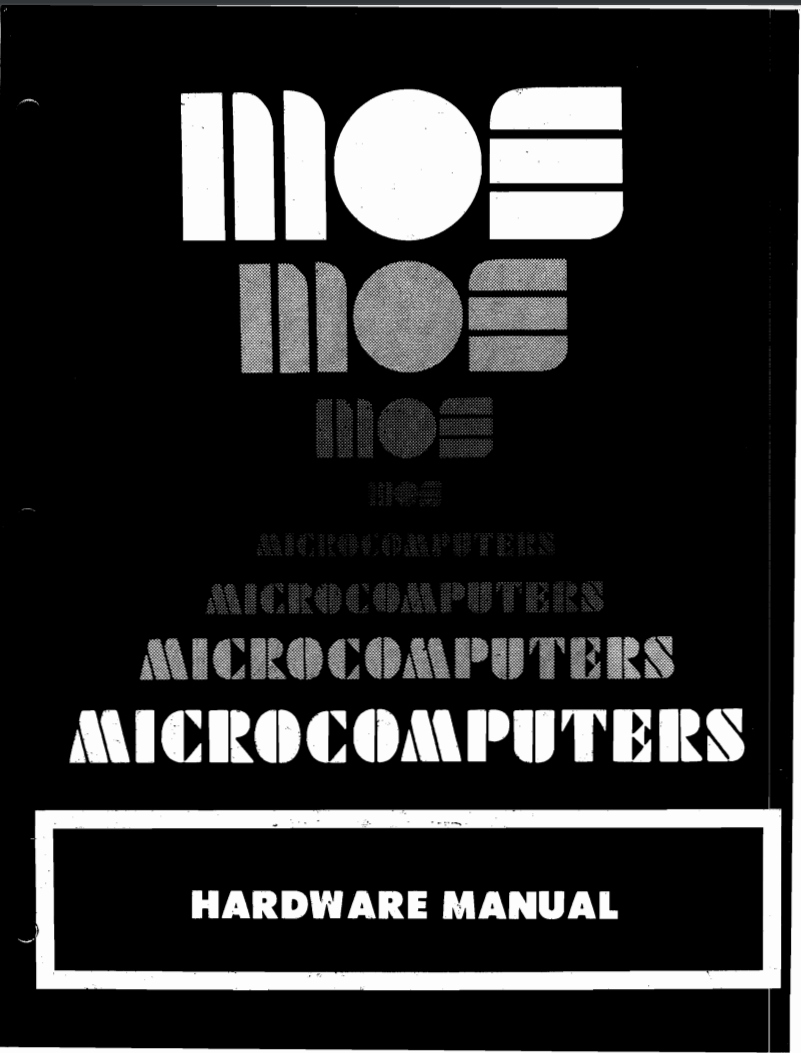
\includegraphics[width=0.25\textwidth]{images/mos-hw-manual.png}
\end{figure}

\section{Nintendo Entertainment System}
Konzole Nintendo Entertainment System, často zkracována jako NES, je osmibitový zábavní počítačový systém firmy Nintendo, který byl vydán nejprve v Japonsku jako Family Computer (FC, \enquote{Famicom}). První verze je ukázaná na obrázku~\ref{fig:nes}. V~České republice je tento systém znám především díky mnoha klonům (\enquote{televizní hry na žlutých kazetkách}), které byly levnější a~dostupnější než oficiální systém. Tyto klony používaly kopie původního hardwaru, poté se objevily hardwarové emulátory založené na ASIC, které celou konzoli zmenšili do jednoho čipu (proto přezdívány NES-on-a-chip). Tato kapitola má za úkol popsat především technické specifikace systému --- zájemce o~podrobnou historii NES lze odkázati na Wikipedii~\cite{Wikipedia:NES}~\cite{Wikipedia:famiclone} a~článek~\cite{Svara:polystation}.

\begin{figure}[ht!]
	\centering
	\caption{Konzole Nintendo Entertainment System (foto \copyright~2016, Evan-Amos)}
	\label{fig:nes}
	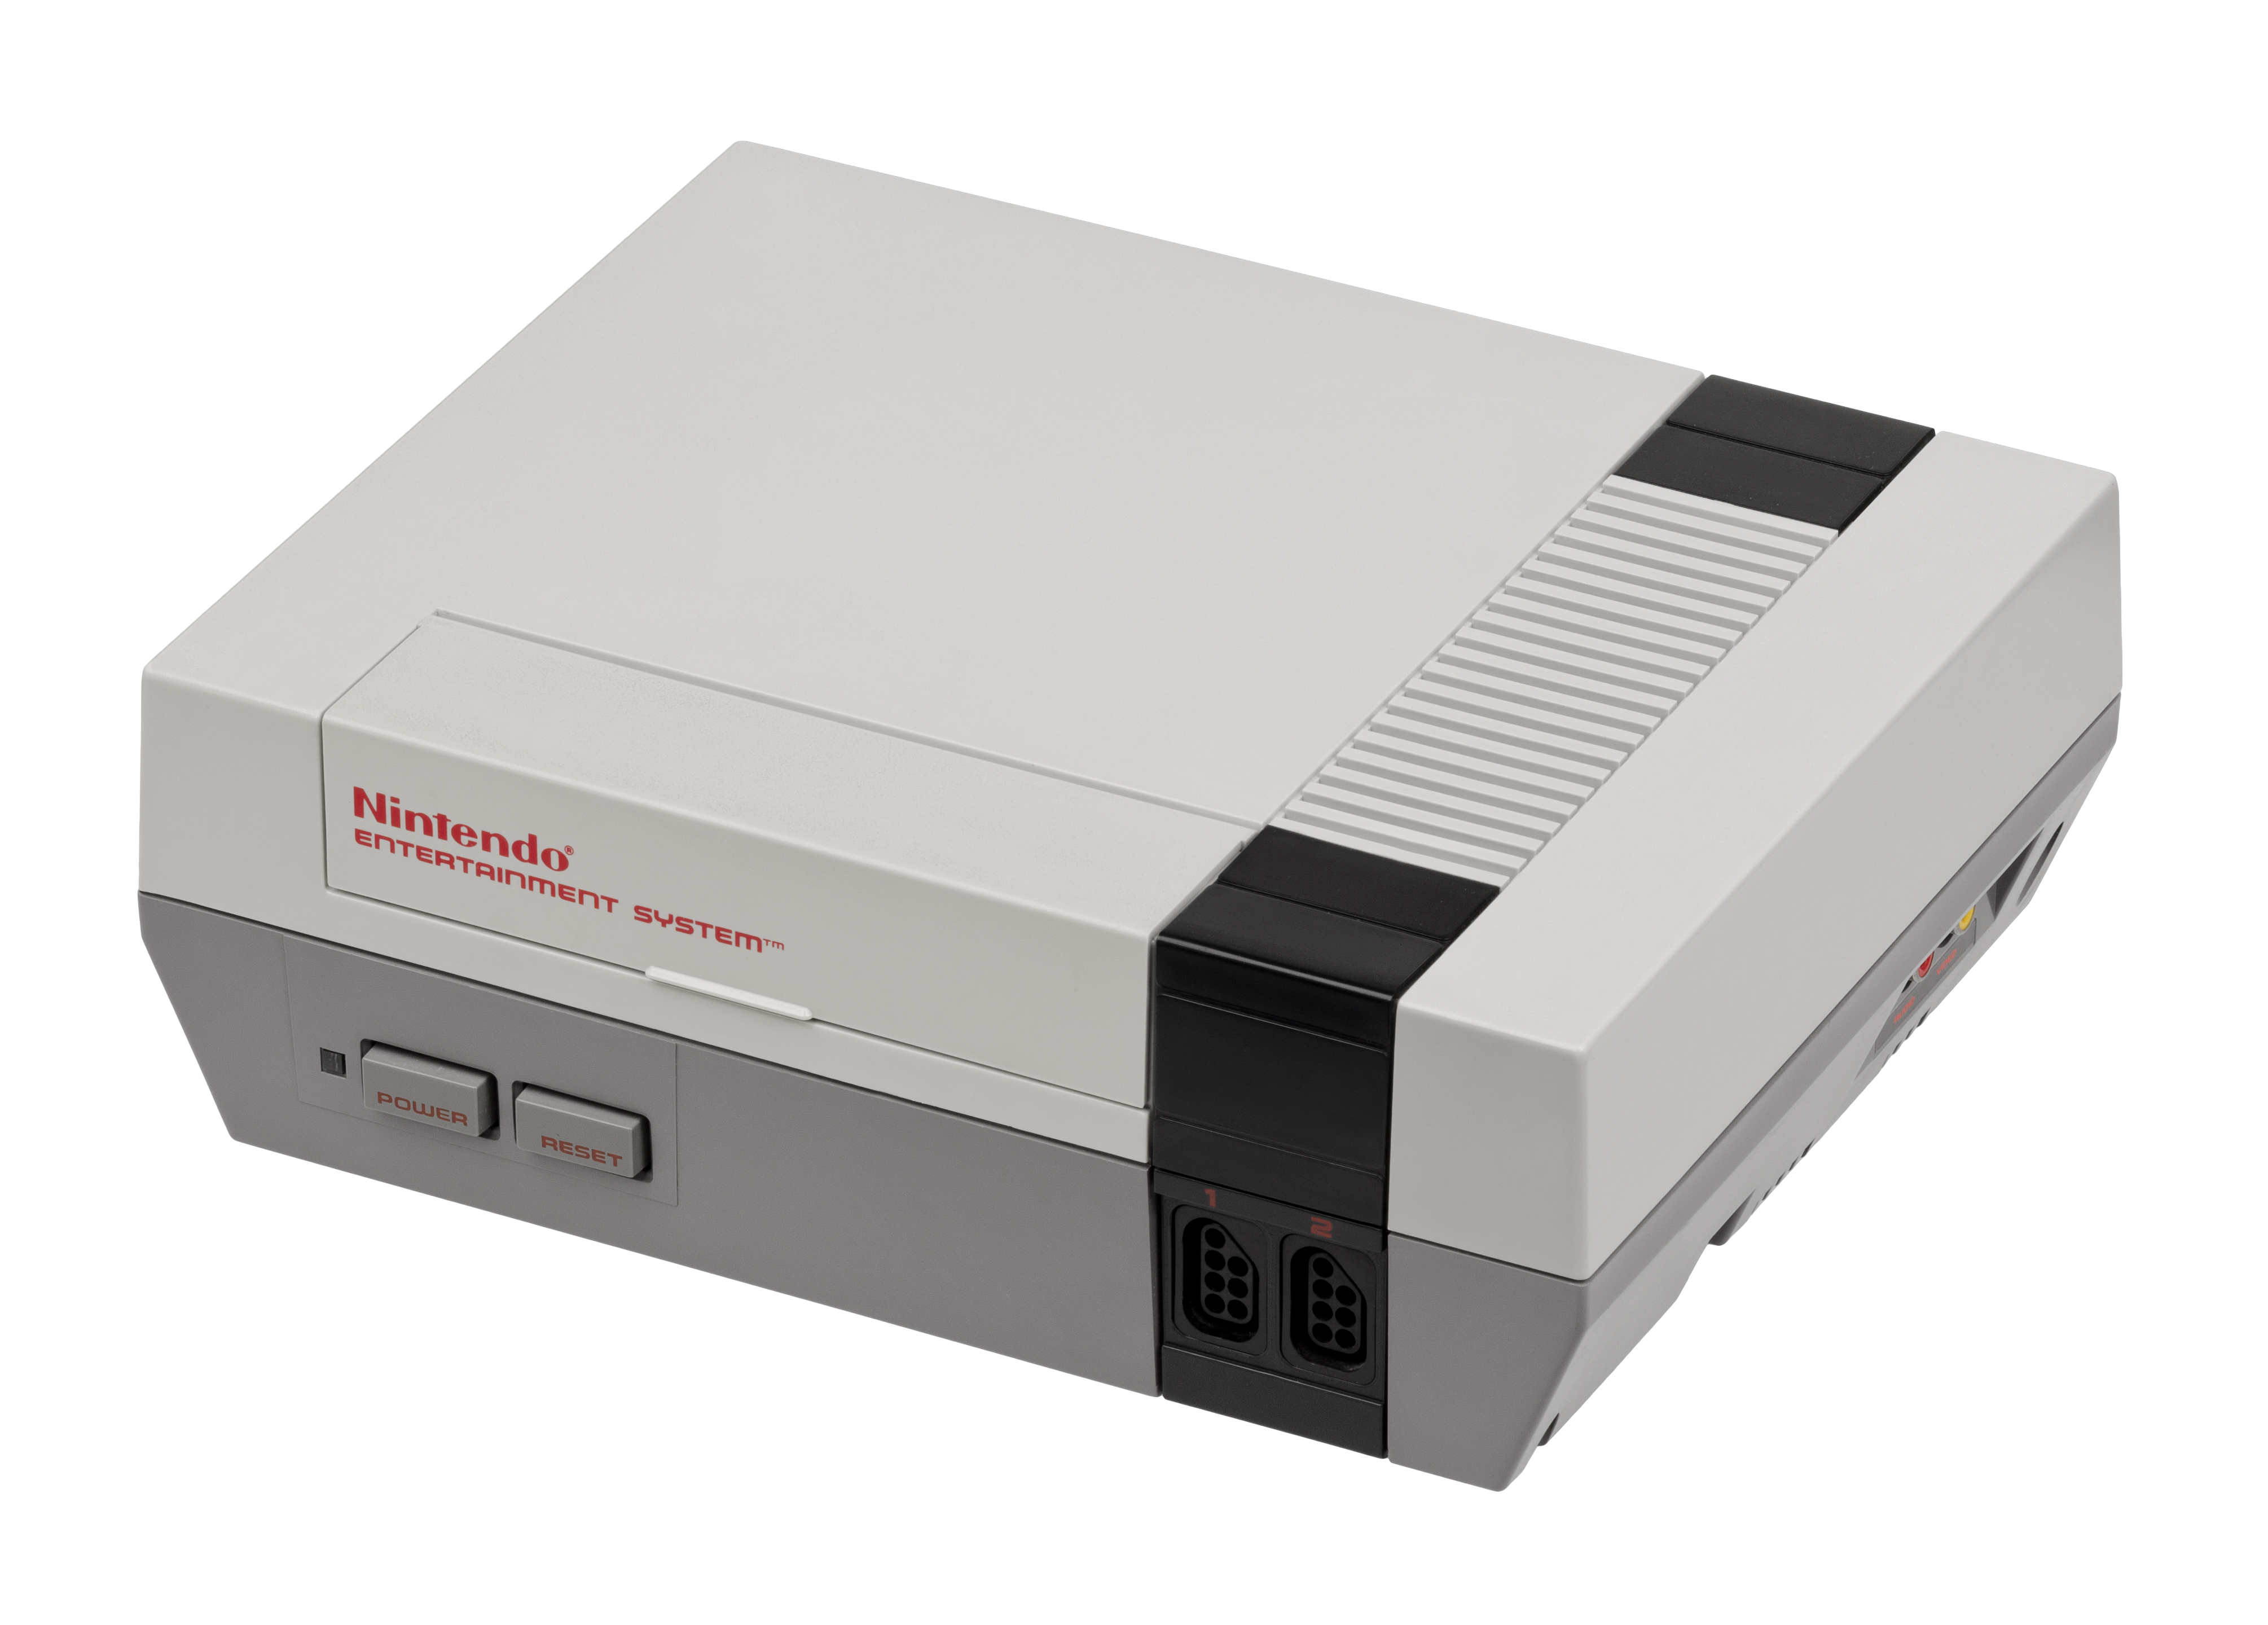
\includegraphics[width=0.4\textwidth]{images/nes.jpg}
\end{figure}


Systém se skládá z několika hlavních komponent, které spolu komunikují pomocí dvou sběrnic. Nejprve jsou představeny sběrnice a~k~nim připojené komponenty, jež jsou později rozebrány podrobněji.

\subsection{Hlavní sběrnice}
Hlavní sběrnice, kterou ilustruje obrázek~\ref{fig:nes-hlavnisbernice}, je adresována 16~bity a~přenáší 8~datových bitů. Komunikaci na hlavní sběrnici řídí pouze procesor~\emph{2A03}, který obsahuje i~řadič přímého přístupu do pamětí (DMA). Tudíž neexistuje (a~ani není potřebná) žádná forma arbitrace.

\begin{figure}[ht!]
	\centering
	\caption{~Hlavní sběrnice konzole NES}\label{fig:nes-hlavnisbernice}
	% Kód pro renderování sběrnice byl inspirován příspěvkem od uživatele Ignasi na StackExchange.
	% https://tex.stackexchange.com/questions/319864/how-to-improve-my-draw-for-i2c-bus
	\begin{tikzpicture}[
		master/.style={draw, rounded corners, fill=mastercomponent, minimum height=15mm, minimum width=2.5cm},
		slave/.style={draw, rounded corners, fill=slavecomponent, minimum height=10mm, minimum width=2.5cm},
		slot/.style={draw, rounded corners, fill=interface, minimum height=10mm, minimum width=2.5cm}
		]
		
		\node[master] (m) {CPU (2A03)};
		\node[slave, below right=3mm and 7mm of m] (s1) {RAM};
		\node[slave, right= 3mm of s1] (s2) {APU};
		\node[slave, right= 3mm of s2] (s3) {PPU (2C02)};
		\node[slot, right= 3mm of s3] (s4) {I/O};
		
		\draw[thick] (m)--(m-|s4) node[above]{Hlavní sběrnice};
		\foreach \i in {1,2,3,4}{
			\draw[fill=black] (s\i)--(s\i|-m) circle (2pt);
		}
		
		\node[slave, below left=of s4] (gamepak) {Game Pak};	
		\draw[dashed] (s4)--(gamepak);
		
		
		\node[slave, below=of s4] (periferie) {Periferie};	
		\draw[dashed] (s4)--(periferie);
	\end{tikzpicture}
\end{figure}

Procesor má k~dispozici 2~kB paměti RAM. Přímo v~procesoru se nachází čip pro generování zvuku, přezdívaný jako Audio Processing Unit (APU).  Na sběrnici se dále nachází grafický čip \emph{2C02}, označovaný jako Picture Processing Unit (PPU). Jako poslední je na sběrnici několik vstupně-výstupních (I/O) rozhraní: slot pro paměťové médium typu kazeta (cartridge), obchodně označovaná jako Game~Pak, pomocí níž se distribuoval veškerý software pro konzoli, a~porty pro periferie, především herní ovladače.

\begin{note}[APU a~hlavní sběrnice]
	APU, ačkoliv je součástí procesorového čipu, také komunikuje na hlavní sběrnici. Proto je na obrázku~\ref{fig:nes-hlavnisbernice} uveden jako další zařízení na sběrnici.
\end{note}

\subsection{Grafická sběrnice}
Systém obsahuje i~vedlejší sběrnici adresovanou 14~bity (celkem tedy 16~kB adresovatelného prostoru), kde komunikaci řídí PPU. Schematicky je znázorněna na obrázku~\ref{fig:nes-grafickasbernice}. Tato sběrnice je zcela oddělena od hlavní. Sběrnice obsahuje paměť video RAM (VRAM, také označována jako CIRAM) o~kapacitě 2~kB. Do paměťového prostoru je dále mapována RAM obsahující barevnou paletu. V~systému existuje ještě paměť OAM (Object Attribute Memory), která obsahuje seznam spritů a~informace potřebné k~jejich zobrazování. Ta je ale není připojena ke sběrnici, nýbrž přímo k~čipu PPU.

\begin{definition}[Sprite]
	Sprite (počeštěně sprajt) je dvourozměrný obrázek, který bývá integrován do větších scén. Termín pochází z~dob, kdy se zvlášť vykreslovalo pozadí a~právě sprity, které často představovaly herní postavičky a~asociované předměty (zbraně, náboje a~další). To je případ i~konzole NES, která pro sprity měla dedikovanou paměť OAM.
\end{definition}

\begin{note}[Přístup CPU na grafickou sběrnici]
	Přestože není procesor přímo připojený na grafickou sběrnici, může na ní nepřímo komunikovat přes registry PPU (\$2006 a \$2007), které jsou mapovány na hlavní sběrnici (a~tím i~do adresního prostoru CPU). Tyto registry se používají i~pro přístup během DMA.
\end{note}

\begin{figure}[ht!]
	\centering
	\caption{~Grafická sběrnice konzole NES}\label{fig:nes-grafickasbernice}
	% Kód pro renderování sběrnice byl inspirován příspěvkem od uživatele Ignasi na StackExchange.
	% https://tex.stackexchange.com/questions/319864/how-to-improve-my-draw-for-i2c-bus
	\begin{tikzpicture}[
		master/.style={draw, rounded corners, fill=mastercomponent, minimum height=15mm, minimum width=2.5cm},
		slave/.style={draw, rounded corners, fill=slavecomponent, minimum height=10mm, minimum width=2.5cm},
		slot/.style={draw, rounded corners, fill=interface, minimum height=10mm, minimum width=2.5cm}
		]
		
		\node[master] (m) {PPU (2C02)};
		\node[slave, below right=3mm and 7mm of m] (s1) {VRAM};
		\node[slave, right= 6mm of s1] (s2) {Paletová RAM};
		\node[slave, below=of m] (s3) {OAM};
		
		\draw[thick] (m)--(m-|s2.east) node[above]{Grafická sběrnice};
		\foreach \i in {1,2}{
			\draw[fill=black] (s\i)--(s\i|-m) circle (2pt);
		}
		\draw[dashed] (m) -- (s3);
		
	\end{tikzpicture}
\end{figure}

\section{Procesor 6502}
Základem NES je klon procesoru \emph{6502}, označený jako \emph{2A03}. Tato podkapitola popisuje původní variantu procesoru a~specifika klonu jsou rozebrány v~samostatné podkapitole~\ref{sec:2A03}.

\subsection{Historie}
Procesor 6502 navrhla firma MOS Technology v~roce 1975. Na procesoru pracoval tým, který původně navrhoval mikroprocesor Motorola 6800. 6502 vznikl jako levnější a~rychlejší alternativa procesoru od Motoroly pod vedením Chucka Peddla~\cite{computer-history-museum:chuck-peddle}, která zachovává hardwarovou kompatibilitu. Cílem bylo umožnit využití i~v~projektech, kde by jinak byla levnější diskrétní logika~\cite{mos:hw-manual}. Ve své podstatě jde o~aplikaci programovatelného počítače (definovaného v~kapitole~\ref{chap:predstaveni-problematiky}) v~praxi --- funkce zařízení lze změnit pouze výměnou programu, což byl i~jediný požadavek při přechodu z~konkurenční Motoroly; upravit program pro ISA 6502.

\subsection{Interakce procesoru s~prostředím}
Na úvod, jak se píše v~hardwarovém manuálu~\cite{mos:hw-manual}, je vhodné se zabývat, v~jakém prostředí procesor bude pracovat~a jak s~ním bude interagovat. Prostředím je myšlen systém, který bude procesorem řízen. Procesor 6502 s okolím komunikuje pomocí jedné systémové sběrnice, která obsahuje 16~adresních vodičů, 8~datových vodičů a~signál R/W, který signalizuje zdroj dat vzhledem k~procesoru. Logická jednička (napětí větší než 2,4~V) signalizuje čtení procesorem, logická nula pak zápis procesorem. Okolí procesoru je tvořeno několika komponentami, ty jsou součástí adresního prostoru CPU, který je znázorněn v~tabulce~\ref{tab:cpu-adresniprostor}.

Adresní prostor je v~terminologii produktové řady MCS650X rozdělen na stránky, což představuje rozsah adresovatelný jedním bajtem (256 adres). Index v~rámci stránky zajišťuje spodní bajt, index stránky poté horní bajt. Z~toho vyplývá, že stránek je také 256. Znalost tohoto faktu je klíčová pro pochopení důvodu existence speciálního zero-page adresního režimu, který je vysvětlen v~podkapitole~\ref{sec:6502-adresni-rezimy}.

\begin{table}[ht!]
	\centering
	\caption{~Adresní prostor CPU}\label{tab:cpu-adresniprostor}
	\begin{tblr}{|Q[c,m]|Q[c,m]|}
		\hline
		Adresní rozsah & Zařízení \\
		\hline[2pt]
		\$0000–\$07FF & RAM \\
		\hline
		\$0800–\$1FFF & Zrcadlo \$0000–\$07FF \\
		\hline
		\$2000–\$2007 & Registry PPU \\
		\hline
		\$2008–\$3FFF & Zrcadlo \$2000–\$2007 \\
		\hline
		\$4000–\$4017 & Registry APU a I/O \\
		\hline
		\$4018–\$401F & Nepoužíváno \\
		\hline
		\$4020–\$FFFF & Game Pak \\
		\hline
	\end{tblr}
\end{table}

Komunikace je řízena dvoufázovými systémovými hodinami, v~první fázi se vystaví adresa na sběrnici (předstih), v~druhé fázi dochází k~přenosu dat. Z~těchto dvou fází se pak skládá celý procesorový cyklus~\cite{mos:hw-manual}. Příklad komunikace směrem k~procesoru (čtení) je znázorněn na obrázku~\ref{fig:6502-casovani-cteni}. Dle dokumentace je pro 1MHz hodiny garantováno, že adresa bude stabilní 300~ns po náběžné hraně první fáze; naopak je požadováno, aby data byla platná alespoň 100~ns před sestupnou hranou druhé fáze hodin.

\begin{figure}[ht!]
	\centering
	\caption{~Časování čtení procesoru}\label{fig:6502-casovani-cteni}
	\begin{tikztimingtable}[%
		timing/dslope=0.1,
		timing/.style={x=5ex,y=3ex},
		x=5ex,
		timing/rowdist=4ex,
		timing/name/.style={font=\sffamily\scriptsize}
		]
		\signal{CLK $\phi1$}     & L l H H H L L L h \\
		\signal{CLK $\phi2$}     & H L L L H H H L  \\
		\signal*{R/W}            & L l h 6H \\
		\signal[15:0]{ADRESA}    & 1.5D{...} U 4.5D{adresa do paměti} U \\
		\signal[7:0]{DATA}       & 5.5Z 2D{data z paměti} u  \\
		\extracode
		\begin{pgfonlayer}{background}
			\begin{scope}[semitransparent ,semithick]
				\vertlines[black,dotted]{1.0,2.0,...,7.5}
				\vertlines[gray,dotted]{0.5,1.5,...,8.0}
			\end{scope}
		\end{pgfonlayer}
	\end{tikztimingtable}
\end{figure}

Kromě systémové sběrnice existuje další způsob komunikace, a~to je přerušení. Všechny procesory v~produktové řadě MCS650X obsahují celkem tři vstupy reprezentující různá přerušení: RST, IRQ a~NMI.

\subsection{Architektura}
Po diskusi vnější komunikace procesoru je vhodné se zabývat jeho architekturou, a~nejen instrukční sadou, ale i~implementačními detaily tam, kde je to nutné. Architekturou se zabývá především softwarový manuál~\cite{mos:sw-manual}.

Procesor 6502 je osmibitový, jelikož pracuje se slovem o~velikosti osmi bitů. ISA procesoru 6502 je střadačově orientovaná, pracovní registr je totiž právě pouze střadač (akumulátor). ISA definuje adresu jako 16bitové číslo ve formátu little-endian, jako první je tedy vždy uváděn nejméně významný bajt (LSB). ISA také definuje několik adresních režimů, z~toho jeden speciální, zero-page režim, který slouží jako částečná náhrada absence více registrů a~efektivně činí z~první paměťové stránky pomyslnou zápisníkovou paměť.

Nejprve je potřeba analyzovat datovou cestu pro pochopení, jaký hardware mají jednotlivé instrukce k~dispozici. Dále adresní režimy, jelikož struktura a~délka instrukcí a~instrukční cyklus s~nimi pevně souvisí.

\begin{note}[Značení adresních bajtů]
	Jelikož je adresa uváděna po bajtech a~obsahuje právě dva bajty, bylo zavedeno v~rámci příruček firmy MOS označení ADL (address low) pro nejméně významný (nižší) bajt adresy a~ADH (address high) pro nejvíce významný (vyšší) bajt. Tohoto značení se drží i~bakalářská práce.
\end{note}

\subsubsection{Datová cesta}
Procesor 6502 obsahuje ve své datové cestě několik registrů. V~tabulce~\ref{tab:6502-registry} je uveden popis registrů s~velikostmi, často používanými zkratkami a~popisem obsahu.

\begin{table}[ht!]
	\centering
	\caption{~Registry procesoru 6502}\label{tab:6502-registry}
	\begin{tblr}{|Q[c,m]|Q[c,m]|Q[c,m]|X[c,m]|}
		\hline
		Registr & Zkratka & Velikost (bit) & Obsah \\
		\hline[2pt]
		programový čítač & PC & 16 & adresa instrukce ke zpracování \\
		\hline
		střadač (akumulátor) & A & 8 & zpracovávané hodnoty \\
		\hline
		ukazatel zásobníku & S & 8 & adresa vrcholu zásobníku \\
		\hline
		indexovací registr X & X & 8 & adresní offset \\
		\hline
		indexovací registr Y & Y & 8 & adresní offset \\
		\hline
		registr příznaků & P & 8 & výsledky provedení ALU operací a~stav CPU \\ 
		\hline
	\end{tblr}
\end{table}

Střadač v ISA 6502 má podobný účel jako v~jiné střadačové architektuře. Jedná se o~jediný univerzální registr, všechny operace musí být prováděny přes zásobník (kromě načítání a~ukládání, což zvládají i~indexovací registry). To znamená aritmetické a~logické operace, porovnávání, změny hodnot. Střadač je implicitním úložným místem pro výsledky operací.

Zásobník architektury 6502 je fixován na adresách \$0100--\$01FF. Jeho kapacita je tedy 256 bajtů a~roste odshora dolů. Se zásobníkem se manipuluje pomocí dedikovaných instrukcí, je možné na zásobník uložit střadač nebo obsah příznakového registru. Adresa vrcholu zásobníku je v~registru S. 

Indexovací registry slouží primárně jako zdroj offsetu pro adresní režimy s~indexací. Fungují jako čítač, existují instrukce pro jejich inkrementaci (INX, INY), dekrementaci (DEX, DEY) a~porovnávání hodnot s~hodnotou v~paměti (CPX, CPY). Jelikož se ale jejich hodnota načítá z~paměti a~lze do paměti i~uložit, mohou sloužit jako programem využitelné pomocné registry.

Příznakový registr obsahuje 7 využívaných příznaků. Jejich popis je v~tabulce~\ref{tab:6502-flags}. Index označuje pořadí bitu (zprava), do kterého se daný příznak ukládá při použití instrukce PHP. Příznakem, který ve fyzickém registru není implementován, je B. Tento příznak je viditelný pouze při operaci přenosu registru příznaků do zásobníku a~jeho hodnota záleží na tom, která operace přenos do zásobníku vyvolala. Přenos je vyvolán dvěma způsoby:

\begin{itemize}
	\item softwarově (instrukce BRK a~PHP): hodnota B je 1,
	\item hardwarově (přerušení): hodnota B je 0.
\end{itemize}

Tím, že registr B nemá hardwarovou reprezentaci, je jeho hodnota ignorována při navrácení příznaků ze zásobníků.

\begin{table}[ht!]
		\centering
		\caption{Popis příznakového registru procesoru 6502\label{tab:6502-flags}}.
		\begin{tblr}{|Q[c,m]|Q[c,m]|X[c,m]|}
			\hline
			Index & Příznak &  Popis \\
			\hline[2pt]
			0 & C & Operace vygenerovala přenos. \\
			\hline
			1 & Z & Zpracovávaná hodnota je nulová. \\
			\hline
			2 & I  & Maska přerušení (hodnota 1: přerušení maskováno) . \\
			\hline
			3 & D & Režim BCD (hodnota 1: režim je aktivní). \\
			\hline
			4 & B & Příznak \enquote{break}. Neexistuje fyzicky. \\
			\hline
			5 & - & Nepoužito. \\
			\hline
			6 & V & Operace vyvolala přetečení. \\
			\hline
			7 & N & Zpracovávaná hodnota je záporná (má-li sedmý bit má hodnotu 1) \\
			\hline
		\end{tblr}
	\end{table}

Procesor dále obsahuje pomocné registry pro dočasné ukládání paměti a~dat (programově nepřístupné; používané při přístupu na sběrnici). Nedílnou součástí je pak také aritmeticko-logická jednotka, ve které probíhají nejen konkrétní výpočty požadované instrukcemi, ale i~pomocné výpočty například pro zjištění absolutní adresy při vyhodnocování skoků.

\subsubsection{Základní adresní režimy}
\label{sec:6502-adresni-rezimy}
Základní adresní režimy pracují pouze s~pevnými adresními hodnotami. Patří mezi ně implikovaný režim, okamžitý režim, absolutní režim, režim nulté stránky a~relativní režim.

Nejjednodušší adresní režim se skládá pouze z~operačního znaku (OZ, anglicky opcode), který jednoznačně identifikuje příslušnou instrukci. Sama instrukce implikuje, s~jakými daty se bude pracovat, proto je tento režim nazván \emph{implikovaný} a~taková instrukce má vždy 1 bajt. Struktura a~příklad instrukce je znázorněn na obrázku~\ref{fig:6502-adr-impl}.

\begin{figure}[ht!]
	\centering
	\caption{~Struktura instrukce implikovaného adresního režimu s~příkladem instrukce Clear Interrupt Disable Bit (CLI)}\label{fig:6502-adr-impl}
	
	\begin{bytefield}[bitheight=\widthof{~Sign~},
		boxformatting={\centering\small\ttfamily}]{8}
		\bitbox[]{8}{}    		   & \bitheader[endianness=little]{0,7} \\
		\bitbox[]{8}{}    		   & \bitbox{8}[bgcolor=bfcommon]{OZ} \\
		\bitbox[]{8}{}    		   & \bitheader[endianness=little]{0,7} \\
		\bitbox[]{8}{CLI} & \bitboxes*{1}[bgcolor=bfcommonlight]{01011000}
	\end{bytefield}
\end{figure}

Další adresní režim pracuje s~konstantní hodnotou, která je uváděná ihned za operačním znakem. To znamená, že se zpracovávaná hodnota nemusí načítat z~paměti pomocí adresy, ale nachází se přímo ve zpracovávaném kódu. Označuje se jako \emph{okamžitý} (immediate) a~instrukci tak tvoří dva bajty. Příklad je uveden na obrázku~\ref{fig:6502-adr-imm}; instrukce AND provede logický součin hodnoty v~akumulátoru s~konstantou \$42.

\begin{figure}[ht!]
	\centering
	\caption{~Struktura instrukce okamžitého adresního režimu s~příkladem instrukce AND Memory with Accumulator (AND)}\label{fig:6502-adr-imm}
	
	\begin{bytefield}[bitheight=\widthof{~Sign~},
		boxformatting={\centering\small\ttfamily}]{8}
		\bitbox[]{8}{}    		   & \bitheader[endianness=little]{0,7,8,15} \\
		\bitbox[]{8}{}    		   & \bitbox{8}[bgcolor=bfcommon]{OZ} & \bitbox{8}[bgcolor=bfcommon]{konstanta} \\
		\bitbox[]{8}{}    		   & \bitheader[endianness=little]{0,7,8,15} \\
		\bitbox[]{8}{AND} & \bitboxes*{1}[bgcolor=bfcommonlight]{00101001} & \bitboxes*{1}[bgcolor=bfcommonlight]{01000010}
	\end{bytefield}
\end{figure}

Adresní režim, který již pracuje s~hodnotami adres, se označuje jako \emph{absolutní}. Součástí instrukce v~tomto režimu je přímá hodnota adresy, kde se nachází kýžená data. Instrukce je tedy 3 bajtová. Formát instrukce i~s~příkladem je na obrázku~\ref{fig:6502-adr-abs}; demonstrovaná instrukce načte do akumulátoru hodnotu ze~zařízení v~adresním prostoru procesoru na adrese \$102.

\begin{figure}[ht!]
	\centering
	\caption{~Struktura instrukce absolutního adresního režimu s~příkladem instrukce Load Accumulator (LDA)}\label{fig:6502-adr-abs}
	
	\begin{bytefield}[bitheight=\widthof{~Sign~},
		boxformatting={\centering\small\ttfamily}]{8}
		\bitbox[]{8}{}    		   & \bitheader[endianness=little]{0,7,8,15,16,23} \\
		\bitbox[]{8}{}    		   & \bitbox{8}[bgcolor=bfcommon]{OZ} & \bitbox{8}[bgcolor=bfcommon]{ADL} & \bitbox{8}[bgcolor=bfcommon]{ADH} \\
		\bitbox[]{8}{}    		   & \bitheader[endianness=little]{0,7,8,15,16,23}  \\
		\bitbox[]{8}{LDA} & \bitboxes*{1}[bgcolor=bfcommonlight]{10101101} & \bitboxes*{1}[bgcolor=bfcommonlight]{00000010} & \bitboxes*{1}[bgcolor=bfcommonlight]{00000001}
	\end{bytefield}
\end{figure}

Absence univerzálních registrů je částečně suplována existencí adresním režimem \emph{nulté stránky} (zero-page). Adresa, která je uvedena za OZ, je jednobajtová. V~tomto režimu je možné indexovat pouze v~rámci jedné stránky, a~to té první (při indexování od nuly nulté) (adresní rozsah \$0000--\$00FF). Zato však tyto instrukce zabírají dva bajty v~instrukční paměti a~jejich zpracování je rychlejší. Na nultou paměťovou stránku je tak možné nahlížet jako na formu ručně spravované cache~---~v~programátorském manuálu řady MSC6500~\cite{mos:sw-manual} je zdůrazněno, že je program možné optimalizovat přesunem nejčastěji používaných hodnot právě do nulté stránky. Formát je znázorněn na obrázku~\ref{fig:6502-adr-zp}; instrukce Store Accumulator načte do akumulátoru bajt z~první paměťové stránky s offsetem \$42.

\begin{figure}[ht!]
	\centering
	\caption{~Struktura instrukce adresního režimu nulté stránky s~příkladem instrukce Store Accumulator (STA)}\label{fig:6502-adr-zp}
	
	\begin{bytefield}[bitheight=\widthof{~Sign~},
		boxformatting={\centering\small\ttfamily}]{8}
		\bitbox[]{8}{}    		   & \bitheader[endianness=little]{0,7,8,15} \\
		\bitbox[]{8}{}    		   & \bitbox{8}[bgcolor=bfcommon]{OZ} & \bitbox{8}[bgcolor=bfcommon]{ADL} \\
		\bitbox[]{8}{}    		   & \bitheader[endianness=little]{0,7,8,15}  \\
		\bitbox[]{8}{STA} & \bitboxes*{1}[bgcolor=bfcommonlight]{10000101} & \bitboxes*{1}[bgcolor=bfcommonlight]{01000010}
	\end{bytefield}
\end{figure}

\emph{Relativní} adresování je používáno výlučně instrukcemi větvení. Obsahuje pouze jeden adresní bajt, který reprezentuje offset v~dvojkovém doplňku. Vyhodnotí-li se podmínka skoku kladně a~skok se tedy provádí, je hodnota offsetu přičítána k~adrese následující instrukce (než se podmínka skoku vyhodnotí, nachází se již programový čítač na další adrese). V~JSA obecně není nutné uvádět offset explicitně, uvádí se konkrétní adresa, nebo návěští; pomocí těchto údajů je assembler schopen výsledný offset dopočítat. Režim je demonstrován na instrukci Branch On Carry Set na obrázku~\ref{fig:6502-adr-rel} s~offsetem \$42.

\begin{figure}[ht!]
	\centering
	\caption{~Struktura instrukce relativního adresování s~příkladem instrukce Branch On Carry Set (BCS)}\label{fig:6502-adr-rel}
	
	\begin{bytefield}[bitheight=\widthof{~Sign~},
		boxformatting={\centering\small\ttfamily}]{8}
		\bitbox[]{8}{}    		   & \bitheader[endianness=little]{0,7,8,15} \\
		\bitbox[]{8}{}    		   & \bitbox{8}[bgcolor=bfcommon]{OZ} & \bitbox{8}[bgcolor=bfcommon]{offset} \\
		\bitbox[]{8}{}    		   & \bitheader[endianness=little]{0,7,8,15}  \\
		\bitbox[]{8}{BCS} & \bitboxes*{1}[bgcolor=bfcommonlight]{10110000} & \bitboxes*{1}[bgcolor=bfcommonlight]{01000010}
	\end{bytefield}
\end{figure}

\subsubsection{Adresní režimy s~indexací}
Složitější adresní režimy přinášejí další možnost přístupu k~datům v~paměti. Do této chvíle byly uvedeny pouze takové režimy, které disponují pouze pevně stanovenou adresou. Často je však nutné adresy měnit, nebo vytvářet zcela dynamicky. Takový typ adres označuje manuál~\cite{mos:sw-manual} jako počítané adresy. Pro práci s~počítanými adresami obsahuje ISA speciální adresní režimy využívající indexovací registry: absolutní režim s~indexací a~režim nulté stránky s~indexací.

\begin{example}[Kopírování souvislých dat bez indexace]
Jedním ze základních řídicích struktur programovacích jazyků jsou cykly, které mohou posloužit jako nástroj pro práci s~bloky dat. Typickým příkladem nechť je kopírování dat z~jednoho paměťového místa na jiné. Ve střadačové architektuře se provádí načtením do střadače a~uložením.

Byla-li by implementace provedena pouze za použitím pevných adres, muselo by se pro každé paměťové místo uvést instrukci načtení i~instrukci zápisu. Vytváří-li se adresy dynamicky, je možné provést operace v~cyklu. Ačkoliv existuje způsob úpravy pevných adres za běhu programu pomocí techniky samomodifikujícího se kódu (viz stranu 72 manuálu~\cite{mos:sw-manual}), představují adresní režimy s~indexací elegantnější alternativu nevyžadující přepisovatelnou instrukční paměť.
\end{example}

Nechť je jako první uveden \emph{absolutní adresní režim s~indexací}. Tento režim přidává absolutnímu režimu možnost přičíst k~původní adrese i~offset z~registru X, nebo Y; dle zvoleného registru se tak jedná o~dva různé adresní režimy. Adresa pevně určená instrukcí je nazývaná jako základová (base). Výsledná adresa je vypočtena jednoduše: $zakladova\_adresa + offset$. Struktura je stejná jako u standardního absolutního režimu na obrázku~\ref{fig:6502-adr-abs}.

Podobně jako u~standardních režimů existuje možnost pracovat pouze s~nultou stránkou, k~tomu~účelu slouží \emph{režim nulté stránky s~indexací}. Struktura instrukce je opět stejná jako na obrázku~\ref{fig:6502-adr-zp}. V~tomto režimu nedochází k~překročení paměťových stránek při přičtení indexu, horní bajt je ignorován a~výpočty tak efektivně probíhají v~modulu \$100. Výpočet tedy probíhá jako: $(zakladova\_adresa + offset) \mod 256$. Kromě instrukcí LDX a~STX, kdy jsou k~dispozici oba indexovací registry k~výběru, je tento režim použitelný pouze s~registrem X.

\subsubsection{Nepřímé adresování}
V~architektuře 6502 existuje ještě \emph{nepřímé adresování}, které umožňuje pracovat s~ukazateli, namísto s~přímou hodnotou adresy. Takové režimy jsou dva, indexovaný-nepřímý a nepřímý-indexovaný. Názvy režimů jsou odvozené podle pořadí, ve kterém se přičítá index.

První zmíněný režim, \emph{indexovaný-nepřímý}, pracuje s~jednobajtovou adresou následovanou po operačním znaku. Tato adresa je základ ukazatele do nulté stránky. K~základu se přičte hodnota indexovacího registru X. Součet probíhá opět v modulu 256, vyšší bajt je totiž zahazován. Vznikne tak výsledný ukazatel, který směřuje na místo nacházející se v~nulté stránce, které obsahuje první bajt kýžené adresy. Ta je opět uspořádána ve formátu nižší bajt a~vyšší bajt. Příklad na obrázku~\ref{fig:6502-adr-idx-ind} ukazuje variantu instrukce STA v~indexovaném-nepřímém režimu. Samotný OZ se základem ukazatele je umístěn v~instrukční pamětí na adrese \$F000. K~základu \$42 je přičten obsah registru X \$10. Výsledkem je adresa \$52, na které se již nachází 16bitová konečná adresa. Instrukce STA v~popsaném příkladě tedy uloží hodnotu akumulátoru až na adresu zjištěnou v~posledním kroku: \$3412.

\begin{figure}[ht!]
	\centering
	\caption{~Struktura instrukce indexovaného-nepřímého režimu s~příkladem instrukce STA}\label{fig:6502-adr-idx-ind}
	
	\begin{bytefield}[bitheight=\widthof{~Sign~},
		boxformatting={\centering\small\ttfamily}]{8}
		\bitbox[]{8}{} & \bitheader[endianness=little]{0,7,8,15} \\
		\bitbox[]{8}{\$F000:} & \bitbox{8}[bgcolor=bfcommon]{OZ} & \bitbox{8}[bgcolor=bfcommon]{základ ukazatele} & \bitbox[]{8}{} & \bitbox{8}[bgcolor=bfaux]{X} \\

		\bitbox[]{8}{} & \bitboxes*{1}[bgcolor=bfcommonlight]{10000001} & \bitbox{8}[bgcolor=bfcommonlight]{\$42} & \bitbox[]{8}{} & \bitbox{8}[bgcolor=bfauxlight]{\$10} \\ \\ \\

		\bitbox[]{8}{Výpočet:} & \bitbox{8}[bgcolor=bfcommonlight]{\$42} & \bitbox{1}[]{+} & \bitbox{8}[bgcolor=bfauxlight]{\$10} \\

		\bitbox[]{8}{} & \bitheader[endianness=little]{0,7,8,15} \\ \bitbox[]{8}{\$52:} & \bitbox{8}[bgcolor=bfcommon]{ADL} & \bitbox{8}[bgcolor=bfcommon]{ADH} \\
		
		\bitbox[]{8}{} & \bitbox{8}[bgcolor=bfcommonlight]{\$12} & \bitbox{8}[bgcolor=bfcommonlight]{\$34}
	\end{bytefield}
\end{figure}

Druhý režim, \emph{nepřímý-indexovaný}, funguje podobně, ale přičítání indexu probíhá až v~druhém kroku a~používá se registr Y. Po operačním znaku následuje hodnota ukazatele, která se již nemění. Ukazuje do nulté stránky, kde se nachází dvojbajtový základ konečné adresy. K~základu se přičte hodnota registru Y. Vznikne tak konečná adresa, se kterou může daná instrukce dále pracovat. Příklad opět na instrukci STA je uveden na obrázku~\ref{fig:6502-adr-ind-idx}. Tentokrát bude hodnota akumulátoru uložena na adresu \$3422.

\begin{figure}[ht!]
	\centering
	\caption{~Struktura instrukce nepřímého-indexovaného režimu s~příkladem instrukce STA}\label{fig:6502-adr-ind-idx}
	
	\begin{bytefield}[bitheight=\widthof{~Sign~},
		boxformatting={\centering\small\ttfamily}]{8}
		\bitbox[]{8}{} & \bitheader[endianness=little]{0,7,8,15} \\
		\bitbox[]{8}{\$F000:} & \bitbox{8}[bgcolor=bfcommon]{OZ} & \bitbox{8}[bgcolor=bfcommon]{ukazatel} & \bitbox[]{8}{} & \bitbox{8}[bgcolor=bfaux]{X} \\
		
		\bitbox[]{8}{} & \bitboxes*{1}[bgcolor=bfcommonlight]{10000001} & \bitbox{8}[bgcolor=bfcommonlight]{\$42} & \bitbox[]{8}{} & \bitbox{8}[bgcolor=bfauxlight]{\$10} \\
		
		\bitbox[]{8}{} & \bitheader[endianness=little]{0,7,8,15} \\ \bitbox[]{8}{\$42:} & \bitbox{8}[bgcolor=bfcommon]{ADL} & \bitbox{8}[bgcolor=bfcommon]{ADH} \\
		
		\bitbox[]{8}{} & \bitbox{8}[bgcolor=bfcommonlight]{\$12} & \bitbox{8}[bgcolor=bfcommonlight]{\$34} \\ \\ \\
		
		\bitbox[]{8}{Výpočet:} & \bitbox{8}[bgcolor=bfcommonlight]{\$3412} & \bitbox{1}[]{+} & \bitbox{8}[bgcolor=bfauxlight]{\$10} \\
	\end{bytefield}
\end{figure}

Existuje ještě jeden nepřímý režim, označovaný jako \emph{nepřímý absolutní}. Tento režim je použit pouze instrukcí skoku (JMP). Princip je podobný jako u~zmíněných nepřímých režimů s~tím rozdílem, že nedochází k~přičítání indexu. Instrukce se skládá z~operačního znaku a~dvou adresních bajtů, které fungují jako 16bitový ukazatel na výslednou adresu, na kterou se má skočit. V~příkladu na obrázku~\ref{fig:6502-adr-ind} instrukce JMP skočí na adresu uloženou na adrese \$2010, jejíž hodnota je \$FA55 --- skok bude tedy proveden na adresu \$FA55.

\begin{figure}[ht!]
	\centering
	\caption{~Struktura instrukce JMP využívající nepřímý absolutní adresní režim s~příkladem skoku na adresu \$FA55}\label{fig:6502-adr-ind}
	
	\begin{bytefield}[bitheight=\widthof{~Sign~},
		boxformatting={\centering\small\ttfamily}]{8}
		\bitbox[]{8}{} & \bitheader[endianness=little]{0,7,8,15,16,23} \\
		\bitbox[]{8}{\$F000:} & \bitbox{8}[bgcolor=bfcommon]{OZ} & \bitbox{8}[bgcolor=bfcommon]{ukazatel (LO)} & \bitbox{8}[bgcolor=bfcommon]{ukazatel (HI)} \\
		
		\bitbox[]{8}{} & \bitboxes*{1}[bgcolor=bfcommonlight]{01101100} & \bitbox{8}[bgcolor=bfcommonlight]{\$10} & \bitbox{8}[bgcolor=bfcommonlight]{\$20} \\
		
		\bitbox[]{8}{} & \bitheader[endianness=little]{0,7,8,15} \\ \bitbox[]{8}{\$2010:} & \bitbox{8}[bgcolor=bfcommon]{ADL} & \bitbox{8}[bgcolor=bfcommon]{ADH} \\
		
		\bitbox[]{8}{} & \bitbox{8}[bgcolor=bfcommonlight]{\$55} & \bitbox{8}[bgcolor=bfcommonlight]{\$FA} \\
	\end{bytefield}
\end{figure}

\begin{example}[Využití nepřímého adresování]
Nepřímé adresování má mnoho různých využití. U indexovaného-nepřímého se jedná především o~práci se seznamem adres. Tento seznam může uchovávat například adresy tlačítek herních ovladačů, ze kterých se periodicky vyčítá stav. Nepřímý-indexovaný pak může sloužit k~modifikaci chování volaného podprogramu. Úpravou hodnoty registru Y bude podprogram pracovat s~jiným offsetem v~odkazované paměti.
\end{example}

\subsubsection{Instrukční cyklus}
\label{sec:6502-instrukcni-cyklus}
Instrukční cyklus odpovídá standardnímu cyklu procesoru, jako uvádí prof. Kubátová v~\cite{Kubatova2018:SAP}; fetch (načtení instrukce), decode (dekódování instrukce), execute (provedení instrukce). Dekódování je věnována zvláštní pozornost v~podkapitole~\ref{sec:6502-dekodovani-instrukci}. Standardně je součástí běhu navíc počáteční nastavení při spuštění a~ošetření příčiny přerušení; právě tomuto je věnována zvláštní pozornost v~podkapitolách~\ref{sec:6502-reset} a~\ref{sec:6502-preruseni}.

\begin{figure}[ht!]
	\centering
	\caption{~Instrukční cyklus procesoru}\label{fig:6502-instrukcni-cyklus}
	\begin{tikzpicture}[node distance=2cm] 
		\tikzstyle{akce} = [rectangle, minimum width=4cm, minimum height=1cm, text centered, draw=black, fill=fcaction]
		\tikzstyle{startstop} = [rectangle, rounded corners, minimum width=3cm, minimum height=1cm,text centered, draw=black, fill=fcstart]
		\tikzstyle{vetveni} = [diamond, minimum width=3cm, minimum height=1cm, text centered, draw=black, fill=fcbranch]
		\tikzstyle{arrow} = [thick,->,>=stealth]
		
		\node (start) [startstop] {Start};
		\node (IC) [vetveni, below of=start] {Přerušení?};
		\node (IS) [akce, right of=IC, xshift=3cm] {Obsluha přerušení};
		\node (IF) [akce, below of=IC] {Načtení instrukce};
		\node (ID) [akce, below of=IF] {Dekódování instrukce};
		\node (EX) [akce, below of=ID] {Provedení instrukce};
		\node (aux) [left=2cm of IC] {};
		
		\draw [arrow] (start) -- (IC);
		\draw [arrow] (IC) -- node[anchor=south] {ano} (IS);
		\draw [arrow, <-] (IF) -| (IS);
		\draw [arrow] (IC) -- node[anchor=east] {ne} (IF);
		\draw [arrow] (IF) -- (ID);
		\draw [arrow] (ID) -- (EX);
		\draw [arrow] (EX) -| (aux);
		\draw [arrow] (aux) -- (IC);
	\end{tikzpicture} 
\end{figure}

Přesné dodržení instrukčního cyklu nemusí být u~emulace nutné, dokonce bývá zvykem velkou část cyklu zjednodušit pro dosažení většího výkonu tak, že se pracuje pouze na úrovni instrukcí. Jelikož je ale v~systému komponent více, je nutné se zabývat alespoň délkou trvání jednotlivých instrukcí, aby nedocházelo ke ztrátě synchronizace. 

Délka zpracování instrukce je vázána především na její typ a podtyp --- pohybuje se od 2 do 7 (8 v~případě nedokumentovaných instrukcí) strojových cyklů. Instrukce totiž existují ve více variantách v~závislosti na použitém adresním režimu. Každý podtyp je jednoznačně identifikován operačním znakem. To znamená, že pro stejnou instrukci existuje více různých operačních znaků, lišících se pouze v~adresním režimu. Je tedy možné délku zpracování odvodit pouze na základě operačního znaku.

Existují však výjimky. U~některých instrukcí pracujících s~pamětí může dojít k~překročení paměťové stránky, což způsobí provedení jednoho strojového cyklu navíc. To se týká adresních režimů pracujících s~indexy, konkrétně absolutního režimu s~indexací pro registry X i~Y. Týká se to i~nepřímého-indexovaného režimu, ten totiž také přičítá hodnotu registru k~16bitové adrese s~možností překročení stránky. Indexovaný-nepřímý režim již nedovoluje překročení paměťové stránky (horní bajt je vždy ignorován a~k~přenosu do vyššího řádu tak nedochází); jej se to již tedy netýká.

Poslední výjimkou jsou instrukce větvení. Dojde-li ke kladnému vyhodnocení podmínky, musí se vykonat jeden strojový cyklus navíc; to je způsobeno nutností přičíst offset k~programovému čítači. Dojde-li navíc k~překročení paměťové stránky, musí se kvůli přičtení přenosu provést ještě další strojový cyklus. Abych to shrnul, je-li proveden skok, který navíc překračuje stránku, provedou se navíc celkem dva strojové cykly.

\begin{note}[6502 a pipelining]
	Procesor 6502 zároveň provádí více činností --- operace na vnitřní sběrnici provádí souběžně s~operacemi na vnější sběrnici. Zatímco na vnější sběrnici se připravuje operační znak a~příslušné adresy, na vnitřní probíhají výpočty (inkrementace programového čítače, operace na aritmeticko-logické jednotce a~další). Díky pipeliningu je možné instrukce zpracovat v~méně cyklech. Pro účely emulace to však není relevantní a~zájemci si mohou o~problematice více přečíst v~manuálu~\cite{mos:sw-manual}.
\end{note}

Podrobný rozpis vykonávaných úkonů při zpracování instrukcí je s~přesností na strojové cykly uveden na v~příloze A hardwarového manuálu~\cite{mos:hw-manual}.

\subsubsection{Dekódování instrukcí}
\label{sec:6502-dekodovani-instrukci}
Každá instrukce je jednoznačně identifikována včetně příslušného adresního režimu pomocí operačního znaku. V~případě 6502 je tento operační znak vždy 8bitový.  Každá instrukce je prováděna v~několika strojových cyklech.  Index strojového cyklu je uchováván v~čítači a~v~dokumentaci je označován písmem T s indexem (například T1 pro první cyklus). Dvojice operační znak a~index jsou dekódovány v~programovatelném logickém poli (Programmable Logic Array, PLA).  Právě použití PLA způsobilo existenci takzvaných neoficiálních instrukcí, viz podkapitola~\ref{sec:6502-rozsirena-instrukcni-sada}.

PLA slouží k~efektivní implementaci kombinační logiky.  Oproti klasické paměti PLA nevyžaduje záznam pro každou možnou adresu, výstupy jsou řízeny hradly AND a~OR, které implementují logickou funkci v~disjunktivní normální formě~\cite{Wikipedia:PLA}. Takto je možné efektivně zakódovat funkci obsahující hodnoty \enquote{don't care}, aniž by muselo dojít k~duplikaci řádků. Právě díky hodnotám don't care může jeden záznam reagovat na více různých vstupů, v~případě řadiče 6502 jsou vstupem operační kódy. Mají-li se stejná operace vykonat pro více operačních kódu, je to implementováno právě takto.

Příklad několika záznamů je uveden v~tabulce~\ref{tab:6502-PLA}, kde například operační znak \$AC ve strojovém cyklu T3 způsobí načtení hodnoty ze sběrnice do registru Y. Operační znak \$AF však vlivem hodnot don't care způsobí načtení do dvou registrů: A a~X.  Operační znaky s~více funkcemi jsou neoficiální a~jejich bližší popis je v~podkapitole~\ref{sec:6502-rozsirena-instrukcni-sada}.

\begin{table}[ht!]
	\centering
	\caption{Ukázka záznamů v~PLA procesoru 6502~\cite{Steil2008:illegal-opcodes}}\label{tab:6502-PLA}
	\begin{tblr}{|Q[c,m]|Q[c,m]|X[c,m]|}
		\hline
		Maska & Cyklus &  Popis \\
		\hline[2pt]
		\texttt{10101100} & T3 & Načti do registru Y. \\
		\hline
		\texttt{101011X1} & T3 & Načti do registru A. \\
		\hline
		\texttt{1010111X} & T3 & Načti do registru X. \\
		\hline
		
	\end{tblr}
\end{table}

\subsubsection{Instrukční sada}
\label{sec:6502-instrukce}
Instrukční sadu procesoru je možné rozdělit do několika skupin dle jejich účelu. Každá instrukce se pak dělí dle adresních režimů, které používá; to určuje i~délku vykonávání ve strojových cyklech a~také říká, zdali dojde při překročení paměťové stránky k~vykonání dalšího strojového cyklu. Nakonec je u~každé instrukce známo, jaké příznaky procesoru nastavuje. Instrukce má pro použití v~JSA symbolické textové označení, které se označuje jako mnemonika (mnemonic); příklady takových označení již byly uvedeny u~adresních režimů, například STA pro Store Accumulator. Instrukční sada je popsána nejen v~oficiálních manuálech, ale i~v~mnoha přehledných dokumentech, které jsou k~dispozici na webu; tato kapitola je tedy věnována analýze formátu takových dokumentů a~ukázce pár instrukcí.

Popis instrukcí většinou bývá ve formě tabulky. První tabulkou je přehled operačních znaků, kde řádky odpovídají vyšším čtyřem bitům OZ a~sloupce nižším bitům. Další tabulka je poté věnována popisům jednotlivých instrukcí. Příkladem je tabulka~\ref{tab:6502-instr-priklad}, ve které je mnemonika instrukce, seznam příznaků a~stručný popis.

\begin{table}[ht!]
	\centering
	\caption{Ukázka popisu instrukcí logických operací}\label{tab:6502-instr-priklad}
	\begin{tblr}{|Q[c,m]|Q[c,m]|Q[c,m]|Q[c,m]|Q[c,m]|Q[c,m]|Q[c,m]|X[c,m]|}
		\hline
		Instrukce & N & Z & C & I & D & V & Popis \\
		\hline[2pt]
		AND & \checkmark  & \checkmark & - & - & - & - & Provede logický součin střadače a~hodnoty z~paměti. \\
		\hline
		EOR & \checkmark  & \checkmark & - & - & - & - & Provede úplnou disjunkci (XOR) střadače a~hodnoty z~paměti. \\
		\hline
		ORA & \checkmark  & \checkmark & - & - & - & - & Provede disjunkci střadače a~hodnoty z~paměti. \\
		\hline
		
	\end{tblr}
\end{table}

\subsubsection{Rozšířená instrukční sada}
\label{sec:6502-rozsirena-instrukcni-sada}
Kromě oficiálních instrukcí, tedy takových, které byly popsány v~oficiálních manuálech od výrobce, existuje i~\enquote{skrytá} množina instrukcí, označována jako neoficiální nebo nelegální. Tyto instrukce nebyly brány v~potaz při návrhu a~jejich existence je důsledkem principu, který byl použit pro dekódování instrukcí (dekódování probíhá v druhém kroku instrukčního cyklu, viz podkapitola~\ref{sec:6502-instrukcni-cyklus}). Nejprve je tedy vhodné pochopit, jak funguje dekódování instrukcí u~procesoru 6502, což vysvětluje podkapitola~\ref{sec:6502-dekodovani-instrukci}.

Některé instrukce jsou prostou kombinací více instrukcí. Tyto instrukce bývají stabilní a~používají je i~některé oficiální hry. Například hra \emph{Disney's Aladdin}~\cite{Nesdev:illegal-opcodes} z~roku 1994 používá instrukci SLO, která kombinuje ASL (aritmetický posuv vlevo) a~ORA (disjunkce střadače s~paměťovou hodnotou). Dále je často používána instrukce LAX, která  načte hodnotu do akumulátoru i~do registru X. Příklad, jak taková instrukce funguje, je popsán v~podkapitole~\ref{sec:6502-dekodovani-instrukci}.

Další instrukce nastavují příznaky zvláštním způsobem, popřípadě jsou nestabilní (výsledek je dán fyzikálními jevy, například teplotou čipu). Poslední skupina instrukcí zastaví instrukční cyklus a~je vyžadován restart. Tyto instrukce jsou označovány jako JAM, KIL, HLT. Zastavení instrukčního cyklu je způsobeno nenastavením čítače taktů zpět na první index, procesor se tak zacyklí. 

\subsubsection{Počáteční stav}
\label{sec:6502-reset}

Má-li být emulace věrohodná, je třeba ctít stav po restartu zařízení. Tabulka~\ref{tab:6502-restart} popisuje obsah registrů po restartu. Nejdůležitější je hodnota programového čítače, bez korektního nastavení jeho hodnoty se začne program vykonávat z~nesprávné adresy.

Po spuštění dojde k~7cyklové inicializaci, nakonec se provede instrukce skoku (JMP) na adresu nacházející se ve vektoru resetu \$FFFC--\$FFFD.

\begin{table}[ht!]
	\centering
	\caption{Stav registrů 6502 po restartu}\label{tab:6502-restart}
	\begin{tblr}{|Q[c,m]|Q[c,m]|}
		\hline
		Registr & Hodnota \\
		\hline[2pt]
		P & \$34 \\
		\hline
		A & 0 \\
		\hline
		X & 0 \\
		\hline
		Y & 0 \\
		\hline
		PC & dle vektoru na adresách \$FFFC--\$FFFD \\
		\hline
	\end{tblr}
\end{table}

\subsubsection{Obsluha přerušení}
\label{sec:6502-preruseni}
Přerušení se dá použít mimo jiné pro synchronizaci systémových komponent. Toho využívá například PPU pro oznámení procesoru, že bylo dosaženo konce zobrazitelné oblasti obrazovky. Proto je podrobná analýza obsluh přerušení důležitá. Procesor 6502 disponuje dvěma typy přerušení: NMI a~IRQ (BRK). Tabulka~\ref{tab:6502-vektory} ukazuje vektory jednotlivých přerušení, pro úplnost je uveden i~vektor resetu.

\begin{table}[ht!]
	\centering
	\caption{Vektory přerušení a~resetu}\label{tab:6502-vektory}
	\begin{tblr}{|Q[c,m]|Q[c,m]|}
		\hline
		Přerušení & Vektor \\
		\hline[2pt]
		NMI & \$FFFA--\$FFFB \\
		\hline
		IRQ, BRK &  \$FFFE--\$FFFF \\
		\hline
		Reset & \$FFFC--\$FFFD \\
		\hline
	\end{tblr}
\end{table}

Přerušení se liší pouze způsobem vyvolání, postup po aktivaci vnitřního signálu je poté stejný. Vždy se dokončí právě probíhající instrukce, pak se na zásobník zálohuje hodnota registrů PC a P, dojde ke změně hodnoty PC na adresu nacházející ve vektoru přerušení pro daný typ a~nakonec se nastaví příznak masky přerušení. Poté se začne zpracovávat první instrukce rutiny přerušení. Z~přerušení se vystoupí instrukcí RTI (return from interrupt), která obnoví uložené hodnoty ze zásobníku a~navrátí se k~původnímu toku programu.

\subsubsection*{NMI}
Přerušení NMI (non-maskable interrupt) je nemaskovatelné a~vyvolává se stejnojmenným pinem. Časový diagram detekce je na obrázku~\ref{fig:6502-detekce-nmi}. K~detekci dochází v~každé druhé fázi strojového cyklu pomocí hranového detektoru. Signál NMI je aktivní v~logické nule, tudíž k~detekci dochází, pakliže byla hodnota v~minulém cyklu 1 a~současná je 0. Dojde-li k~detekci, je v~první fázi následujícího strojového cyklu procesoru aktivován vnitřní signálu, v~diagramu označen jako \emph{NMI aktivní}. Tento signál zůstává aktivní do doby, než dojde ke zpracování~\cite{Nesdev:cpu-interrupts}.

\begin{figure}[ht!]
	\centering
	\caption{~Detekce přerušení NMI}\label{fig:6502-detekce-nmi}
	\begin{tikztimingtable}[
		timing/dslope=0.1,
		timing/.style={x=5ex,y=3ex},
		x=5ex,
		timing/rowdist=4ex,
		timing/name/.style={font=\sffamily\scriptsize}
		]
		\signal{CLK $\phi1$}     & 1.5L 3H 3L 3H 3L h \\
		\signal {CLK $\phi2$}  & H 3L 3H 3L 3H L  \\
		\signal*{NMI}            & H H 12 L   \\
		\signal{NMI aktivní}    & 7.5L 6.5H \\
		\extracode
		\begin{pgfonlayer}{background}
			\begin{scope}[semitransparent ,semithick]
				\vertlines[black,dotted]{1.0,2.0,...,13.5}
				\vertlines[gray,dotted]{0.5,1.5,...,14.0}
   			    \node (detekce) [anchor=south east,inner sep=0pt,color=red] at (7,-3.5) {detekce};
   			    \node[circle, minimum width = 1cm, draw=red] (boddetekce) at (4, -1.5) {};
   			    \draw[thick,->,>=stealth,color=red] (detekce) -- (boddetekce);
			\end{scope}
		\end{pgfonlayer}
	\end{tikztimingtable}
\end{figure}

\subsubsection*{IRQ}
Přerušení IRQ (interrupt request) se dá vyvolat buďto hardwarově stejnojmenným pinem, nebo softwarově instrukcí BRK.

Hardwarová implementace je zajištěna úrovňovým detektorem a~vyvolání probíhá stejně jako u~NMI s~tím rozdílem, že vnitřní signál zůstává aktivní pouze v~cyklu, ve kterém byl vyvolán. Poté dojde k~další kontrole stavu vnějšího signálu NMI a~není-li v~logické nule, vnitřní signál se deaktivuje~\cite{Nesdev:cpu-interrupts}.

Softwarové přerušení pomocí instrukce BRK provede podobný sled kroků jako při vyvolání hardwarovém s~tím rozdílem, že není automaticky nastaven příznak maska přerušení (I).

\subsubsection*{Zvláštnosti}
Reakce na přerušení a~jeho zpracování je jedním z~příkladů, kde se není možné vyhnout emulaci na úrovni strojových cyklů.

První zvláštností je zpožděná reakce IRQ u~instrukcí manipulujících s~maskou přerušení (NMI se to netýká; to je vyvoláno vždy nehledě na masku přerušení). Dvojcyklové instrukce nejprve vyhodnotí stav přerušení a~poté mění masku. Instrukce pro vymazání masky (CLI) a~přepis příznakového registru hodnotou ze zásobníku (PLP) tedy potenciální čekající přerušení odsunou až do další instrukce. Naopak instrukce RTI nejprve smaže masku a~poté kontroluje, zdali není očekávané přerušení IRQ; může tedy k~opětovnému skoku do rutiny přerušení dojít už po dokončení RTI~\cite{Nesdev:cpu-interrupts}.

Další zvláštností je převážení přerušení (komunitně označováno jako hijacking; únos), které je dáno pseudo-prioritou přerušení: NMI, IRQ, BRK. Dojde-li při prvních čtyřech cyklech zpracovávání instrukce BRK k~vyvolání NMI, bude PC nastaven na hodnotu vektoru NMI, namísto očekávaného vektoru BRK (který je společný s~IRQ). Graficky je chování znázorněno na obrázku~\ref{fig:6502-nmi-brk-prevazeni}. Stejně může dojít ke změně vektoru při souběhu IRQ a~NMI. Podobné chování vykazuje i~souběh IRQ a~BRK, ale vzhledem ke stejnému použitému vektoru se to na zpracování programu nikterak neprojevuje, což tento souběh činí irelevantním pro emulační účely~\cite{Nesdev:cpu-interrupts}.

\begin{figure}[ht!]
	\centering
	\caption{Převážení přerušení BRK přerušením NMI}\label{fig:6502-nmi-brk-prevazeni}
	\begin{tikztimingtable}[
		timing/dslope=0.1,
		timing/.style={x=5ex,y=3ex},
		x=5ex,
		timing/rowdist=4ex,
		timing/name/.style={font=\sffamily\scriptsize}
		]
		\signal{CLK $\phi1$}  & l H L H L H L H L H L H L H L \\
		\signal{CLK $\phi2$}  & H L H L H L H L H L H L H L h \\
		\signal{Instrukce}    & 0.5U 14D{BRK}   \\
		\extracode
		\begin{pgfonlayer}{background}
			\begin{scope}[semitransparent ,semithick]
				\vertlines[black,dotted]{0.5,2.5,...,14}
				\draw[thick, decorate, decoration={brace, mirror}, color=red] (0.5, -5.5) -- (8.5, -5.5);
				\node[color=red] (detekce) at (4.5, -7) {zde může dojít k~převážení přerušením NMI};
			\end{scope}
		\end{pgfonlayer}
	\end{tikztimingtable}
\end{figure}

\subsection{Specifika Ricoh 2A03}
\label{sec:2A03}
Aby se zabránilo porušení patentu, v~hardwaru se přerušilo několik cest tak, aby se učinil desítkový režim procesoru nefunkční. Zároveň byl procesor doplněn o~zvukový syntezátor, který je popisován v~podkapitole~\ref{sec:APU}, a~řadič DMA.

Řadič DMA existuje v~2A03 pouze pro dva účely. Prvním je kopírování obrazových dat pro sprajty využívané komponentou PPU, druhým je kopírování surových zvukových dat komponentou APU. Jelikož bude v~emulátoru implementován pouze první typ, následuje jen popis této funkcionality.

Podtyp DMA pro kopírování sprajtů se označuje jako OAM DMA. Spouští se zápisem do paměťově mapovaného registru procesoru na adrese \$4014. Do registru se zapíše číslo paměťové stránky, která se poté celá překopíruje (256 bajtů) do vnitřní paměti PPU přes registr PPU \$2004 (OAM DATA). Tento zápis trvá 513 cyklů (v~případě jiného zarovnání s~procesorem 514, to je ale náhodné po spuštění, tudíž irelevantní)~\cite{Nesdev:ppu-registers}.

\begin{note}[Důvod existence OAM DMA]
	Data pro sprajty je možné zapisovat i~procesorovým přístupem do registru OAM DATA, což je dobře využitelné pro obnovu části paměti. Avšak vzhledem k~tomu, že na přepisování paměti OAM je jen omezený čas (doba prodlevy mezi snímky; vertical blanking), bylo nutné implementovat rychlejší alternativu pro případ nutnosti přepsání celé paměti OAM.
\end{note}

\section{Grafický čip 2C02}
Nedílnou součástí herní konzole je grafický výstup, tu zajišťuje čip 2C02, přezdívaný jako Picture Processing Unit (PPU). 2C02 je grafickým čipem, který ve své podstatě operuje vždy nad surovými daty, pouze s~nimi umožňuje programátorovi efektivně manipulovat --- jak pozadí, tak sprajty jsou hardwarově renderovány. Tím, že PPU generuje přímo kompozitní signál, je průběh renderování pevně svázán s~rozlišením i~použitým televizním standardem. Každý hodinový takt odpovídá jednomu obrazovému bodu na televizní obrazovce.

Existují dvě varianty specifické pro konkrétní trhy v~závislosti na typu výstupního signálu --- NTSC a PAL. Americká verze konzole (NES), kterou se tato práce zabývá, obsahuje variantu pro standard NTSC. Ačkoliv původní hardware oproti jiným konzolím generoval přímo tento analogový signál~\cite{Nesdev:ntsc}, není třeba se tímto při tvorbě emulátoru zabývat --- pro věrohodnost emulace stačí pouze dodržet rozlišení a~časování a~generovat obraz v~hodnotách RGB, které se i~jednoduše zobrazují na monitoru. Případné převedení do analogového signálu lze udělat dodatečně, což se používá ve formě efektů pro \enquote{zvěrohodnění} zážitku z~hraní na emulátoru.

Jedná o~velice rozsáhlý čip. Analýzu je tedy třeba provést v~několika částech. Nejprve se zjistí, s~jakými daty čip pracuje, poté jak se tento čip ovládá (rozhraní, které je dostupné procesoru) a nakonec i~to, jak s~dostupnými daty čip pracuje.

\subsection{Paměti a~data}
Jak již bylo zmíněno v~úvodu, čip PPU je připojen do dvou sběrnic. Jednak je připojen do hlavní systémové sběrnice, pomocí které procesor 6502 s~čipem PPU komunikuje, což je probíráno v~podkapitole~\ref{sec:ppu-cpu-io}. Dále je připojen do své vlastní sběrnice, na kterou je připojena i~část kazety Game Pak (viz tabulka~\ref{tab:gamepak-mapovani} na straně~\pageref{tab:gamepak-mapovani}). Tabulka~\ref{tab:ppu-pametova-mapa} ukazuje rozdělení adresního prostoru vlastní sběrnice čipu PPU včetně částí zařízení, které jsou běžně v~příslušných rozsazích dostupné. Kromě zvenku přístupných pamětí obsahuje PPU ještě mnoho pracovních registrů, které jsou popsány v~sekci~\ref{ppu:pracovni-registry}.

\begin{table}[ht!]
	\centering
	\caption{Adresní prostor vlastní sběrnice PPU}\label{tab:ppu-pametova-mapa}
	\begin{tblr}{|Q[c,m]|Q[c,m]|X[c,m]|X[c,m]}
		\hline
		Rozsah & Popis & Standardně připojeno \\
		\hline[2pt]
		\$0000--\$0FFF & Pattern table 0 & Paměť CHR~ROM/RAM kazety \\
		\hline
		\$1000--\$1FFF & Pattern table 1 & Paměť CHR~ROM/RAM kazety \\
		\hline
		\$2000--\$23FF & Nametable 0 & Vestavěná videopaměť PPU / vlastní paměť kazety \\
		\hline
		\$2400--\$27FF & Nametable 1 & Vestavěná videopaměť PPU / vlastní paměť kazety \\
		\hline
		\$2800--\$2BFF & Nametable 2 & Vestavěná videopaměť PPU / vlastní paměť kazety \\
		\hline
		\$2C00--\$2FFF & Nametable 3 & Vestavěná videopaměť PPU / vlastní paměť kazety \\
		\hline
		\$3000--\$3EFF & Zrcadla rozsahu \$2000--\$2EFF & Viz zrcadlené oblasti \\
		\hline
		\$3F00--\$3F1F & Paletová RAM & Vestavěná paměť PPU \\
		\hline
		\$3F20--\$3FFF & Zrcadla rozsahu \$3F00--\$3F1F & Viz zrcadlené oblasti \\
		\hline		
	\end{tblr}
\end{table}

Nakonec je čip PPU připojen zvlášť ještě k~paměti OAM obsahující sprajty, viz podkapitola~\ref{sec:ppu-oam}.

\subsubsection{Paletová RAM}
Před další diskusí je třeba popsat, jak funguje práce s~barvami v~konzoli NES. Konzole jako taková má pevně danou množinu barev, kterou může používat. Množina je dána verzí čipu v~závislosti na tom, jestli se generuje přímo kompozitní signál, nebo RGB signál, což používaly především arkádové skříňové automaty. Palety lze vygenerovat v~závislosti na různých nastaveních například nástrojem \url{https://bisqwit.iki.fi/utils/nespalette.php}.

Třebaže je tato množina barev už tak omezená, není možné ji používat v~jednu chvíli celou. Množina aktivních barev je uložena v~RAM integrované přímo v~čipu PPU dostupná na sběrnici na adresách \$3F00--\$3F1F. Tato paměť obsahuje čtyři palety pro pozadí a~další čtyři pro sprajty. Úplně první barva (\$3F00) je také nazývána jako univerzální barva. Každá paleta obsahuje hodnotu tří barev ze zmiňované množiny a~dále jednu barvu, která je zrcadlem univerzální barvy pozadí. Obrázek~\ref{fig:ppu-palety} ukazuje vnitřní uspořádání paletové paměti s~ukázkou možného obsahu. Uctivý čtenář si ráčí všimnout, že první barva palety je vždy stejná, totiž taková, která je obsažena na adrese \$3F00. Jedná se  o~zrcadlo tohoto paměťového místa, a~tudíž první barvu lze zvolit pouze pro všechny palety stejnou; proto také označení univerzální barva.

\begin{note}[Přepis barev pozadí]
	Existuje způsob, jakým lze přinutit čip PPU k~přepsání prvních barev z~palet pozadí namísto zrcadlení univerzální barvy. Jedná se však o~nestandardní postup.
\end{note}

\begin{figure}[htp!]
	\centering
	\caption{Část paletové paměti RAM s~ukázkou hodnot barev z~množiny dostupné pro čip 2C02}\label{fig:ppu-palety}
	
	\begin{bytefield}[bitheight=1.5em, bitwidth=\widthof{\$0000},
		boxformatting={\centering\small\ttfamily}]{4}
				
		\bitbox[]{2}{} & \bitheader{0,3} \\

		\begin{rightwordgroup}{Paleta pozadí 0}
			\bitbox[]{2}{\$3F00:} & \bitbox{1}{\$30} & \bitbox{1}[bgcolor=orange]{\$26}  & \bitbox{1}[bgcolor=red]{\$16} & \bitbox{1}[bgcolor=blue]{\textcolor{white}{\$2C}} 
		\end{rightwordgroup} \\
	
		\bitbox[]{2}{} & \wordbox[]{1}{...} \\

		\begin{rightwordgroup}{Paleta pozadí 3}
			\bitbox[]{2}{\$3F0C:} & \bitbox{1}{\$30} & \bitbox{1}[bgcolor=pixel 1]{\$29} & \bitbox{1}[bgcolor=pixel 2]{\$2C} & \bitbox{1}[bgcolor=pixel 3]{\textcolor{white}{\$0D}}
		\end{rightwordgroup} \\\\

		\begin{rightwordgroup}{Paleta popředí 0}
			\bitbox[]{2}{\$3F10:} & \bitbox{1}{\$30} & \bitbox{1}[bgcolor=violet]{\textcolor{white}{\$13}} & \bitbox{1}[bgcolor=purple]{\$04} & \bitbox{1}[bgcolor=pink]{\$33}
		\end{rightwordgroup} \\
	
		\bitbox[]{2}{} & \wordbox[]{1}{...} \\

		\begin{rightwordgroup}{Paleta popředí 3}
			\bitbox[]{2}{\$3F1C:} & \bitbox{1}{\$30} & \bitbox{1}[bgcolor=yellow]{\$37} & \bitbox{1}[bgcolor=brown]{\textcolor{white}{\$08}} & \bitbox{1}[bgcolor=green]{\$29}
		\end{rightwordgroup} \\
		
	\end{bytefield}
	
\end{figure}

\subsubsection{Pattern table}
Pattern table (volně přeložitelné jako tabulka tvarů) je část paměti typicky obsažené v~kazetě ve počtu dvou po sobě jdoucích tabulek. Zde se ukládají tvary, ze kterých se poté skládá výsledný obraz, ať už v~pozadí, nebo ve formě sprajtu. Každá pattern table obsahuje 256 dlaždic. Diagram jedné pattern table je k~nahlédnutí na obrázku~\ref{fig:ppu-pattern-table}, kde jednotlivé dlaždice jsou označeny jako D následované indexem dlaždice.

\begin{figure}[ht!]
	\centering
	\caption{~Struktura pattern table čipu PPU}\label{fig:ppu-pattern-table}
	
	\begin{bytefield}[bitheight=1.5em, bitwidth=0.15em,
		boxformatting={\centering\small\ttfamily}]{256}
		\bitheader[endianness=little]{0,16,32,48,64,80,96,112,128,144,160,176,192,208,224,240} \\
		
		% Vytvoření pattern table pomocí vnořeného cyklu.
		% Natlačení na jeden řádek je třeba, aby \LaTeX nevkládal \par.
		% Pozor: to platí i pro \skippedwords, jinak je taky šoupnuté.
		\newcounter{rowIndex}
		\newcounter{tileIndex}
		\newcounter{tileIndexCalculated}
		\forloop{rowIndex}{0}{\value{rowIndex} < 4}{\forloop{tileIndex}{0}{\value{tileIndex} < 16}{\ifx\tileIndex>0 & \fi\setcounter{tileIndexCalculated}{\value{tileIndex}+\value{rowIndex} * 16}\bitbox{16}{D\arabic{tileIndexCalculated}}} \\}\skippedwords \\
		
		% Poslední řádek.
		\forloop{tileIndex}{240}{\value{tileIndex} < 256}{\ifx\tileIndex>0 & \fi \bitbox{16}{D\arabic{tileIndex}}} \\ 	
	\end{bytefield}
\end{figure}

Každá dlaždice je reprezentována dvěma v~paměti po sobě jdoucími částmi. Každá část má 8~bajtů, dohromady má tedy dlaždice 16 bajtů. Každý bajt jedné části představuje řádek obrázku; každý bit poté představuje část hodnoty pixelu. Poněvadž se dlaždice skládá ze dvou částí, je pro každý pixel definována dvoubitová hodnota. Dolní bit této hodnoty reprezentuje bit z~první části; horní bit pak ten z~druhé části. Hodnota pixelu se používá pro výběr barvy z~aktivní palety --- celkem jsou k~dispozici čtyři různé barvy, z~toho první barva je pro všechny palety stejná. Princip skládání hodnot pixelu je znázorněn na obrázku~\ref{fig:ppu-pattern-tile}, kde je ukázán i~potenciální výsledný obrázek, pokud by se používala paleta pozadí 3 z~obrázku~\ref{fig:ppu-palety}.

\begin{figure}[htp!]
	\centering
	\caption{Ukázka složení částí dlaždic ve výsledný obraz za použití palety pozadí 3 z~obrázku~\ref{fig:ppu-palety}}\label{fig:ppu-pattern-tile}
	
	\begin{bytefield}[bitheight=1.5em, bitwidth=1.5em,
		boxformatting={\centering\small\ttfamily}]{8}
		
		\bitbox[]{8}{část 1 (dolní bity)} & \bitbox[]{8}{+} & \bitbox[]{8}{část 2 (horní bity)} \\
		
        \bitheader{0,7} & \bitbox[]{8}{} & \bitheader{0,7} \\
		
		\bitboxes{1}{01100110} & \bitbox[]{8}{}  & \bitboxes{1}{01100110} \\
        \bitboxes{1}{11011111} & \bitbox[]{8}{}  & \bitboxes{1}{10111111} \\
		\bitboxes{1}{10111111} & \bitbox[]{8}{}  & \bitboxes{1}{11111111} \\
		\bitboxes{1}{11111101} & \bitbox[]{8}{}  & \bitboxes{1}{11111111} \\
		\bitboxes{1}{01111010} & \bitbox[]{8}{}  & \bitboxes{1}{01111110} \\
		\bitboxes{1}{00111100} & \bitbox[]{8}{}  & \bitboxes{1}{00111100} \\
		\bitboxes{1}{00011000} & \bitbox[]{8}{}  & \bitboxes{1}{00011000} \\
		\\\\
		
		\bitbox[]{8}{} & \bitbox[]{8}{= složené dvoubitové indexy do palety} & \bitbox[]{8}{} \\\\
		\bitbox[]{8}{} & \bitboxes{1}{03300330} & \bitbox[]{8}{} \\
		\bitbox[]{8}{} & \bitboxes{1}{31233333} & \bitbox[]{8}{} \\
		\bitbox[]{8}{} & \bitboxes{1}{32333333}  & \bitbox[]{8}{} \\
		\bitbox[]{8}{} & \bitboxes{1}{33333323}  & \bitbox[]{8}{} \\
		\bitbox[]{8}{} & \bitboxes{1}{03333230}  & \bitbox[]{8}{} \\
		\bitbox[]{8}{} & \bitboxes{1}{00333300}  & \bitbox[]{8}{} \\
		\bitbox[]{8}{} & \bitboxes{1}{00033000}  & \bitbox[]{8}{} \\
	\end{bytefield}

	\texttt{výsledný obraz} \\

	\def\pixels{
		{0,3,3,0,0,3,3,0},
		{3,1,2,3,3,3,3,3},
		{3,2,3,3,3,3,3,3},
		{3,3,3,3,3,3,2,3},
		{0,3,3,3,3,2,3,0},
		{0,0,3,3,3,3,0,0},
		{0,0,0,3,3,0,0,0}%
	}

	\begin{tikzpicture}[scale=0.5]
		\drawpixels{\pixels}{pixel}
	\end{tikzpicture}
	
\end{figure}

\subsubsection{Nametable}
Nametable je označení pro část videopaměti, která reprezentuje všechna data potřebná pro vykreslení pozadí na jedné obrazovce ($256 \times 240$ pixelů). Skládá se ze dvou částí:

\begin{itemize}
	\item indexy do pattern table (960 bajtů),
	\item tabulka atributů (64 bajtů).
\end{itemize}

Celkem tedy jedna nametable zabírá přesně 1~KiB.

První 960bajtová část definuje, z~jakých dlaždic se bude skládat obraz na pozadí. Každý bajt je indexem do pattern table. Přeneseně řečeno, nametable slouží tedy vyskládání obrazu dlaždicemi z~pattern table. Jak již bylo zmíněno, dlaždice v~pattern table je velká $8 \times 8$ pixelů, tudíž každý bajt v~nametable řídí oblast velikostně odpovídající dlaždici. Pro jeden řádek je tedy potřeba $\frac{256}{8} = 32$~bajtů a~takových řádků bude $\frac{240}{8} = 30$

\begin{note}[Výběr pattern table]
	Pomocí bajtu lze indexovat v~rámci jedné pattern table, ale již nelze vybrat, se kterou se bude pracovat (celkem jsou v~systému dvě). Výběr pattern table pro pozadí se provádí v~regitru PPUCTRL přístupnému procesoru.
\end{note}

V~této chvíli je tedy jasné, jaká dlaždice se kam umístí a~jak vypadá --- každý pixel může nabývat celkem čtyř různých hodnot, tedy čtyř různých barev. Číslo palety, ze které se barvy získávají, určuje právě druhá část nametable; tabulka atributů.

Tabulka atributů se nachází vždy na konci nametable. Každý bajt tabulky určuje indexy palety pozadí pro oblast o~velikosti $32 \times 32$~pixelů, což odpovídá celkem 16 dlaždicím. Tato oblast je rozdělena na čtyři kvadranty, kdy jsou pro každý kvadrant přiděleny dva bity z~příslušného bajtu. Dvěma bity lze přesně indexovat všechny čtyři dostupné palety pro pozadí. Z~toho všeho vyplývá, že je celá scéna představovaná nametable rozdělena na čtverce obsahující $2\times2$~dlaždice, které vždy sdílejí stejnou paletu.

Pořadí indexů v~bajtů přísluší jednotlivým kvadrantům v~tomto pořadí od~nejvyšších dvou bitů: dolní pravý, dolní levý, horní pravý, horní levý.

Velmi pěkná ukázka je k~dispozici na stránce~\cite{Nesdev:attribute-table}

\subsubsection{Object Attribute Memory}
\label{sec:ppu-oam}
Object Attribute Memory, běžně zkracována jako OAM, je zcela oddělená paměť čipu PPU dedikovaná pouze pro ukládání sprajtů. Nachází se mimo obě sběrnice systému, přímo k~této paměti může přistupovat pouze PPU, nebo nepřímo přes registry OAMADDR a~OAMDATA procesor. Paměť OAM má kapacitu 256 bajtů (což odpovídá i~velikosti jedné paměťové stránky). Informace příslušící jednomu sprajtu zabírají 4~bajty; tudíž kapacita odpovídá uložení 64~sprajtů.

Struktura sprajtu není nikterak složitá. První bajt je souřadnice Y (řádek); druhý slouží k~výběru dlaždice z~pattern table, která bude reprezentovat sprajt; třetí obsahuje atributy, kromě výběru indexu palety pro sprajty obsahuje také informace o~překlopení dlaždice a~prioritu sprajtu; čtvrtý obsahuje souřadnici X (sloupec). Další informace jsou přehledně uvedeny na Nesdev~\cite{Nesdev:oam}.

\begin{note}[Existence dvou OAM]
	Kromě výše popsané OAM, označované jako primární, existuje i~další, takzvaná sekundární. Má poloviční kapacitu a~používá se pouze interně pro ukládání sprajtů patřící na daný obrazový řádek. Programátor k~ní tedy nemá přístup a~využívá se jen~a~pouze během procesu renderování.
\end{note}

\subsection{Vnější rozhraní}
\label{sec:ppu-cpu-io}
PPU je řízeno pomocí osmi registrů mapovaných do paměťového prostoru procesoru. Tyto registry jsou zrcadleny po širokém adresním rozsahu, jak bylo uvedeno v~úvodu. Tabulka~\ref{tab:ppu-registry} poskytuje přehled a~stručný popis. Pro podrobnější informace je možné čtenáře opět odkázat na~\cite{Nesdev:ppu-registers}.

\begin{table}[p!]
	\centering
	\caption{Procesorem přístupné registry čipu PPU. Označení \enquote{-} znamená, že se používá celý bajt pro jedinou hodnotu.}\label{tab:ppu-registry}
	\begin{tblr}{|Q[c,m]|Q[c,m]|Q[c,m]|Q[c,m]|X[l,m]|}
		\hline
		Označení & Adresa & Přístup & Bity & Popis bitů \\
		\hline[2pt]
		\SetCell[r=7]{c} PPUCTRL & \SetCell[r=7]{c} \$2000 & \SetCell[r=7]{c} zápis & \SetCell[r=7]{c} \texttt{VPHB SINN} & \texttt{V}: povolení generování NMI \\ \cline{5} & & & & \texttt{P}: režim PPU (0: slave, 1: master) \\ \cline{5} & & & & \texttt{H}: velikost sprajtů (0: $8\times8$, 1: $8\times16$) \\ \cline{5} & & & & \texttt{B}: výběr pattern table pro pozadí (0: první, 1: druhá) \\ \cline{5} & & & & \texttt{S}: výběr pattern table pro sprajty (0: první, 1: druhá) \\ \cline{5} & & & & \texttt{I}: způsob inkrementace indexu do videopaměti (0: přičíst 1, 1: přičíst 32) \\ \cline{5} & & & & \texttt{NN}: základ pro index do videopaměti (0: \$2000, 1: \$2400, 2: \$2800, 3: \$2C00) \\
		\hline
		\SetCell[r=6]{c} PPUMASK & \SetCell[r=6]{c} \$2001 & \SetCell[r=6]{c} zápis & \SetCell[r=6]{c} \texttt{BGRs bMmG} & \texttt{BGR}: Zvýraznění barev (jednobitová hodnota pro modrou, zelenou a~červenou, 1 zvýraznění aktivuje) \\ \cline{5} & & & & \texttt{s}: Povolení sprajtů \\ \cline{5} & & & & \texttt{b}: Povolení pozadí \\ \cline{5} & & & & \texttt{M}: 1: zobrazit sprajty v~levých 8~pixelech obrazovky, 0: skrýt \\ \cline{5} & & & & \texttt{m}: 1: zobrazit pozadí v~levých 8~pixelech obrazovky, 0: skrýt \\ \cline{5} & & & & \texttt{G}: 1: renderovat ve stupních šedi, 0: renderovat barevně \\
		\hline
		\SetCell[r=3]{c} PPUSTATUS & \SetCell[r=3]{c} \$2002 & \SetCell[r=3]{c} čtení & \SetCell[r=3]{c} \texttt{VSO- ----} & \texttt{V}: 1: probíhá VBlank \\ \cline{5} & & & & \texttt{S}: 1: proběhla kolize sprajtu 0 \\ \cline{5} & & & & \texttt{O}: 1: došlo k~přetečení sprajtů \\
		\hline
		OAMADDR & \$2003 & zápis & - & aktuální adresa v~OAM; běžně se nastaví na \$00 a~poté se použije DMA \\
		\hline
		OAMDATA & \$2004 & čtení i~zápis & - & čtení dat z~OAM, nebo zápis na adresu zvolenou pomocí OAMADDR; zápis autoinkrementuje adresu \\
		\hline
		PPUSCROLL & \$2005 & zápis ($2\times$) & - & zápis aktivní adresy na grafické sběrnici (uzpůsobené pro práci s~plynulým posuvem)) \\
		\hline
		PPUADDR & \$2006 & zápis ($2\times$) & - & zápis aktivní adresy na grafické sběrnici \\
		\hline
		PPUDATA & \$2007 & čtení i~zápis & - & čtení i~zápis dat na grafickou sběrnici \\
		\hline
	\end{tblr}
\end{table}

\subsection{Pracovní registry}
PPU obsahuje také dvě skupiny pracovních registrů sloužící k~průběžnému ukládání vyhodnocovaných a~následně vykreslovaných dat, ale i~pro přístup na grafickou sběrnici zvenčí. První skupina souvisí s~přístupem na videopaměti, což je prováděno nejen programátorem, ale i~čipem PPU samotným. Druhá skupina slouží k~vykreslování sprajtů.

\subsubsection{Pozadí a~práce s~videopamětí}
Data pro vykreslování pozadí jsou uložena ve videopaměti (VRAM), se kterou kromě programátora při zápisu do této paměti pracuje i~PPU při vykreslování obrazu na obrazovku televizoru. Pro adresaci v~rámci paměti se používají dva 15bitové registry, tyto registry jsou sdíleny pro obě aktivity; jak modifikace programátorem, tak čtení samotným čipem. Tabulka~\ref{tab:ppu-vram} ukazuje všechny registry používané pro indexaci ve videopaměti a~jejich abstrahovaný význam v~souvislosti s~posuvem souřadnic na obrazovce.

\begin{table}[htp!]
	\centering
	\caption{Pracovní registry pro práci s~videopamětí}\label{tab:ppu-vram}
	\begin{tblr}{|Q[c,m]|Q[c,m]|Q[c,m]|X[l,m]|}
		\hline
		Označení & Popis & Bity & Popis bitů \\
		\hline[2pt]
		\SetCell[r=4]{c} V & \SetCell[r=4]{c} Aktivní adresa do VRAM & \SetCell[r=4]{c} \texttt{yyy NNYY YYYX XXXX} & \texttt{y}: jemný posuv souřadnice~Y \\ \cline{4} & & & \texttt{N}: index nametable ve VRAM \\ \cline{4} & & & \texttt{Y}: hrubý posuv souřadnice~Y \\ \cline{4} & & & \texttt{X}: hrubý posuv souřadnice~X \\
		\hline
        T & Dočasná adresa do VRAM & \texttt{yyy NNYY YYYX XXXX} & Stejný jako u~registru V. \\
		\hline
		X & Jemný posuv souřadnice X & \texttt{xxx} & - \\
		\hline
		W & Indikace pořadí zápisu & \texttt{w} & Hodnota 0 pro první, hodnota 1 pro druhý zápis. \\
		\hline
	\end{tblr}
\end{table}

Registr T je přístupný pomocí registrů \$2000 (PPUCTRL), \$2005 (PPUSCROLL) a~\$2006 (PPUADDR). Slouží k~úpravě programátorem, nepoužívá se pro samotnou indexaci. Do registru PPUCTRL stačí zapsat jednou a~přenáší se do T pouze index nametable. Do zbývajících dvou registrů se musí zapsat dvakrát, oba sdílejí stejný přepínač pořadí (W) a~oba slouží k~úpravě posuvů. Registr PPUSCROLL je zaměřený na úpravu před začátkem vykreslování snímku pro nastavení posuvu v~rámci videopaměti (zjednodušeně řečeno: tímto se nastavuje okno do videopaměti, které je viditelné na obrazovce, díky principu zrcadlení paměti je takto možné zobrazit části více nametable zároveň). Registr PPUADDR je poté zaměřen na práci se surovými daty vkládané do paměti programátorem pomocí registru PPUDATA, pro adresu do dočasného registru T vkládá v~jiném pořadí a~navíc při druhém zápisu rovnou data aktualizuje i~v~aktivním registru V --- počítá se s~tím, že programátor bude do videopaměti přistupovat okamžitě.

Registr V již slouží pro přímou indexaci ve videopaměti. Horizontální posuvy jsou aktualizovány registrem T buďto okamžitě při druhém zápisu do registru PPUADDR, nebo je aktualizován průběžně v~každém obrazovém bodu 257 každého obrazového řádku. Dále je hodnota posuvu souřadnice Y průběžně aktualizována v~obrazovém bodu 256 každého řádku. Vertikální posuvy jsou aktualizovány registrem T poté na konci intervalu VBlank v~bodech 280--304. Nakonec je hodnota V inkrementována dle nastavení v~PPUCTRL vždy při čtení, nebo zápisu do PPUDATA.

Další informace, příklady a~podrobnosti lze nalézt na příslušné stránce Nesdev:~\cite{Nesdev:ppu-scroll}.

Kromě pracovních registrů jsou v~čipu obsaženy i~posuvné registry, sloužící k~ukládání pixelů a~metadat aktuálně vykreslovaných. Jsou to dva 16bitové registry pro vzory zkopírované z~pattern table a~dva 8bitové pro ukládání souvisejících atributů.

\subsubsection{Sprajty}
Pro práci se sprajty kromě hlavní a~vedlejší OAM existuje i~osm párů 8bitových posuvných registrů uchovávající vzory z~pattern table pro 8 sprajtů vykreslovaných na aktivním obrazovém řádku. Dalších osm klopných obvodů uchovává pro tyto sprajty atributy a~osm čítačů uchovává horizontální pozice (souřadnice X).


\subsection{Inicializace po spuštění}
Všechny registry u~PPU je možné po spuštění vynulovat. Dočasné paměti jako OAM a~paletová RAM nemají definovaný stav po spuštění; od programátora se očekává, že tuto paměť korektně inicializuje.

\subsection{Renderování}
Proces renderování obrazu je pevně spjat s~jeho průběžným vykreslováním na obrazovku. Po načtení veškerých potřebných dat do pamětí a~nastavení čipu pomocí registrů je důležité se zabývat, jak čip s~dodanými daty pracuje. Přehledný, komunitou vytvořený, diagram celého procesu včetně operací na pozadí je součástí přílohy~\ref{apx:ppu}.

\subsubsection{Pozadí}
Proces vykreslování pozadí probíhá průběžně během celého televizního snímku. Sekvence kroků se liší dle obrazového řádku. Jelikož jeden hodinový takt odpovídá přesně jednomu obrazovému bodu výstupního signálu, jsou operace PPU pevně svázány s~rozlišením obrazu. Název pro časový úsek odpovídající jednomu obrazovému bodu v~rámci řádku je \emph{cyklus}.

Na viditelných řádcích (0-239) se provádí sled vnitřních (negenerující výstup) i~vnějších (generující výstup) operací. Sled vnitřních operací je uvedený v~tabulce~\ref{ppu:pozadi-cykly}. Pro načtení příslušného řádku jedné dlaždice z~pattern table (dle indexu v~nametable) jsou třeba 4 přístupy do paměti, na tabulce jsou rozepsány pro cykly 1--8. Po provedení přístupů potřebných pro jednu dlaždici dojde k~naplnění vnitřních posuvných registrů, které mohou generovat samotný výstup na obrazovku, což už se týká vnějších operací. K~těm dochází v~cyklech 4--256, kdy se generuje obrazový bod za použití bitů z~naplněných posuvných registrů. To, jaký konkrétní bit se vybere, závisí na hodnotě vnitřního registru uchovávajícího jemný posuv souřadnice X. Registry vykonají posuv a~pokračuje další cyklus. Před výstupem na obrazovku se ještě vybírá mezi pixelem pozadí a~popředí, tomu je věnována sekce~\ref{sec:ppu-priority}.

\begin{table}[ht!]
	\centering
	\caption{Vnitřní operace PPU během viditelných obrazových řádků}\label{tab:ppu-renderovani}
	\begin{tblr}{|Q[c,m]|X[c,m]|}
		\hline
		Cyklus & Operace \\
		\hline[2pt]
		0 & Žádná. \\
		\hline
		1--2 & Načtení bajtu z~nametable; vyhodnocování sprajtů. \\
		\hline
		3--4 & Načtení bajtu z~tabulky příznaků; vyhodnocování sprajtů. \\
		\hline
		5--6 & Načtení bajtu z~první (spodní) části dlaždice z~pattern table; vyhodnocování sprajtů. \\
		\hline
		7--8 & Načtení bajtu z~druhé (horní) části dlaždice z~pattern table; vyhodnocování sprajtů. \\
		\hline
		9--256 & Stejná posloupnost jako pro cykly 1--8. \\
		\hline
		257--320 & Proces načítání dat pro sprajty. \\
		\hline
		321--336 & Načtení prvních dvou dlaždic pro následující řádek (stejně jako v~cyklech 1--8). \\
		\hline
		337--340 & Načítání bajtů z~nametable (účel pro PPU je neznámý, některé mappery, například MMC5, tyto přístupy detekuje za účelem počítání obrazových řádků). \\
		\hline
	\end{tblr}
\end{table}

Po viditelných řádcích následuje řádek 240 (post-renderovací). Od řádku 240 až do předposledního PPU nepřistupuje PPU do videopaměti, avšak příznak intervalu vertikální prodlevy mezi snímky (VBlank) je nastaven až v~prvním cyklu řádku 241, v~ten moment je vyvoláno i~NMI. Od této chvíle je tedy programátor informován o~možnosti bezpečně přistupovat do videopaměti a~může její obsah libovolně upravovat až do řádku 260.

Poslední řádek, označovaný jako 261 (pre-renderovací), provádí stejné paměťové operace, jako se dějí u~viditelných, akorát nedochází k~vykreslování na obrazovku. Zde se připravují vnitřní registry obsahem patřící na první viditelný řádek.

\subsubsection{Popředí}
Vykreslování sprajtů, tedy obsahu popředí, je u~PPU zařízeno hardwarově. Nemusí být tedy vloženy softwarem do průběžně vykreslované videopaměti, stačí správně zavést obrazová data do paměti OAM a~nakonfigurovat hardwarové vykreslování.

Na každém řádku nejprve probíhá proces vyhodnocování, kdy se rozhoduje, které sprajty budou vykresleny na řádku následujícím:
\begin{enumerate}
	\item Inicializace vedlejší OAM hodnotou \$FF.
	\item Přečtení hlavní OAM a~vybrání prvních osm sprajtů, které mají být vykresleny na řádku (dle souřadnice Y, která je obsažena v~prvním bajtu každého sprajtu).
	\item Kontrola, jestli není v~hlavní OAM definováno více než osm aktivních sprajtů na jednom řádku (obsahuje hardwarovou chybu).
	\item Inicializace vykreslovací pipeline.
\end{enumerate}

Samotné vykreslování probíhá souběžně s~pipeline řešící pozadí. V~každém cyklu se dekrementují čítače uchovávající horizontální souřadnice sprajtů pro daný řádek. Je-li nějaký čítač nulový, začne se sprajt postupně vykreslovat pixel po pixelu --- dojde k~postupnému vysouvání dat z~posuvných registrů příslušící danému sprajtu. Je-li aktivních více sprajtů, vybere se ten, který má na výstupu zrovna neprůhledný pixel (nenulová hodnota) a~zároveň má nejmenší index v~paměti, a~pošle se do multiplexeru, kde se vyhodnotí, jestli se vykreslí pixel sprajtu, nebo pozadí, čemuž se věnuje sekce~\ref{sec:ppu-priority}.

\begin{note}[Chyba v~inkrementaci]
Chyba v~kontrole popisovaná v~bodu 3 se projevuje chybnou inkrementací. První sprajt po nalezení osmi aktivních sprajtů se vyhodnotí správně, poté ale autoinkrementace způsobí vyhodnocování jiných bajtů namísto toho uchovávající souřadnici Y. Jedná se právě o~jednu z~chyb, kterou je také nutné emulovat v~případě, že je třeba spouštět software, který se na tyto chyby spoléhá (což je ale velice vzácné; většina programů se na špatně definované či chybné chování nespoléhala).
\end{note}

Podrobnější popis je k~dispozici na stránce~\cite{Nesdev:ppu-sprites}.

\subsubsection{Výběr pixelu k~vykreslení (priority)}
\label{sec:ppu-priority}
Těsně před vykreslením se pixel pozadí a~pixel popředí (sprajtu) účastní rozhodovacího procesu. Pixel pozadí je vždycky ten, který byl zrovna vysunut z~posuvných registrů pozadí. Pixel popředí je pixel patřící takovému sprajtu, který má nejvyšší prioritu dle nejnižšího indexu a~zároveň je neprůhledný-nenulový (jinak se zvolí další sprajt, po vyčerpání všech osmi sprajtů jde na výstup nulová hodnota sprajtu); nebere se ohled na nastavenou prioritu v~atributech sprajtu.

\begin{note}[Zanedbání priorit a~z~toho plynoucí zvláštnosti]
	Jak bylo uvedeno, do rozhodování vstupuje pixel sprajtu, který je neprůhledný a~má nejnižší index, i~když má tento sprajt v~atributech nastaveno, že prioritu má pozadí. Může se tedy stát, že přestože v~seznamu osmi aktivních sprajtů pro obrazový řádek existuje prioritní sprajt, dojde stejně k~vykreslení pozadí, protože se zkrátka priorita sprajtu v~moment vstupu do rozhodovacího procesu nebere v~potaz.
\end{note}

Samotný rozhodovací proces spočívá v~několika krocích, kdy se nejprve kontroluje \enquote{nulovost} pixelu. Nulová hodnota pixelu totiž indexuje v~paletě univerzální barvu pozadí, což je bráno jako transparentní pixel. Nejsou-li žádný z~pixelů nulové, vykreslí se pixel dle nastavené priority v~atributech sprajtu. Tento proces je graficky znázorněn na obrázku~\ref{fig:ppu-vyber-pixelu}.

\begin{figure}[ht!]
	\centering
	\caption{Proces výběru pixelu k~vykreslení}\label{fig:ppu-vyber-pixelu}
	\begin{tikzpicture}[node distance=2cm] 
		\tikzstyle{akce} = [rectangle, minimum width=3.5cm, minimum height=1cm, text centered, draw=black, fill=fcaction]
		\tikzstyle{startstop} = [rectangle, rounded corners, minimum width=3cm, minimum height=1cm,text centered, draw=black, fill=fcstart]
		\tikzstyle{vetveni} = [diamond, aspect=2, minimum width=3.5cm, minimum height=1cm, text centered, draw=black, fill=fcbranch, yshift=0-0.5cm, align=center]
		\tikzstyle{arrow} = [thick,->,>=stealth]
		
		\node (START) [startstop] {Načtení pixelů};
		\node (BOTHZERO) [vetveni, below of=START] {Oba pixely\\nulové?};
		\node (RENDERUC) [akce, right of=BOTHZERO, xshift=3.5cm, align=center] {Vykresli univerzální\\barvu (\$3F00)};
		\node (BGZERO) [vetveni, below of=BOTHZERO] {Pixel pozadí\\nulový?};
		\node (SPRZERO) [vetveni, below of=BGZERO] {Pixel sprajtu\\nulový?};
		\node (PRIOCHECK) [vetveni, below of=SPRZERO] {Kdo má prioritu?};
		\node (RENDERSPR) [akce, left of=PRIOCHECK, xshift=0-3.5cm] {Vykresli pixel sprajtu};
		\node (RENDERBG) [akce, right of=PRIOCHECK, xshift=3.5cm] {Vykresli pixel pozadí};
		\node (STOP) [startstop, below of=PRIOCHECK] {Konec};

		
 		\draw [arrow] (START) -- (BOTHZERO);
		\draw [arrow] (BOTHZERO) -- node[anchor=south] {ano} (RENDERUC);
    	\draw [arrow] (BOTHZERO) -- node[anchor=east] {ne} (BGZERO);
		\draw [arrow] (BGZERO) -- node[anchor=east] {ne} (SPRZERO);
		\draw [arrow] (SPRZERO) -- node[anchor=east] {ne} (PRIOCHECK);
		\draw [arrow] (PRIOCHECK) -- node[anchor=south] {sprajt} (RENDERSPR);
		\draw [arrow] (PRIOCHECK) -- node[anchor=south] {pozadí} (RENDERBG);
		\draw [arrow, <-] (STOP) -| (RENDERBG);
		\draw [arrow, <-] (STOP) -| (RENDERSPR);
		\draw [arrow] (BGZERO) -| node[anchor=south] {ano} (RENDERSPR);
		\draw [arrow] (SPRZERO) -| node[anchor=south] {ano} (RENDERBG);
	\end{tikzpicture} 
\end{figure}

\section{Game Pak}
Hlavním a~jediným nativně podporovaným formátem distribuce softwaru pro konzoli NES byly kazety (cartridge) označované jako Game Pak. Tyto kazety nebyly pouze standardní pamětí typu ROM, obsahovaly i~často velmi sofistikované obvody především pro mapování paměťových segmentů označované jako mappery, které umožňovaly obejít některé hardwarové limitace konzole. Pro účely emulace je také nutné se zabývat formátem souboru, v~jakém se distribuují kopie těchto kazet; bylo totiž nutné uchovat kromě obsahu paměti i~informaci o~přídavných obvodech na kazetě.

Každá kazeta obsahuje paměť pro program, PRG~ROM, volitelně pracovní paměť pro program, PRG~RAM. Tyto jsou mapovány do rozsahu procesoru. Dále obsahuje buďto paměť pouze pro čtení s~grafickými podklady (CHR~ROM), nebo pracovní paměť (CHR~RAM), do které se grafické podklady nahrály za běhu. Tyto paměti jsou mapovány do rozsahu PPU. Standardní mapování kazety do rozsahu CPU a~PPU je uvedeno v~tabulce~\ref{tab:gamepak-mapovani}. Toto mapování také určuje velikost okna, tedy část paměti, která může být najednou viditelná pro CPU či PPU, pakliže mapper umožňuje přepínat paměťové banky.

\begin{table}[ht!]
	\centering
	\caption{Mapování kazety do rozsahu CPU a~PPU}\label{tab:gamepak-mapovani}
	\begin{tblr}{|Q[c,m]|Q[c,m]|}
		\hline
        Rozsah & Mapování \\
        \hline[2pt]
		\SetCell[c=2]{c} CPU \\
		\hline
		\$6000--\$7FFF & PRG~RAM (s~možností zálohování baterií) \\
		\hline
		\$8000--\$BFFF & PRG~ROM banka 0\\
		\hline
		\$C000--\$FFFF & PRG~ROM banka 1 (případně zrcadlo 0)\\
		\hline
		\SetCell[c=2]{c} PPU \\
		\hline
		\$0000--\$0FFF & CHR~ROM/RAM (pattern table 0) \\
		\hline
		\$1000--\$1FFF & CHR~ROM/RAM (pattern table 1) \\
		\hline
		\$2000--\$2FFF & (volitelně) vlastní videopaměť \\
		\hline
	\end{tblr}
\end{table}

U~přepisovatelných pamětí není pevně definována výchozí hodnota; korektně naprogramovaný software se na výchozí hodnoty nespoléhá. U~emulátorů se však často volí hodnota \$00 či \$FF.

\subsection{Mapper}
Každá kazeta obsahovala řídicí desku, která jednotlivé části paměti umisťovala do paměťových prostorů procesoru a~PPU. Jelikož byl výchozí paměťový rozsah nedostačující pro komplexnější hry, umožňovaly sofistikovanější mappery přepínat mezi jednotlivými bankami paměti, což se označuje jako \emph{bankswitching}. Tyto desky byly mnoha typů, jednoduché byly složeny z~diskrétních komponent (deska NROM), složitější obsahovaly zákaznické obvody (ASIC), například deska MMC1 a~její podtypy (SKROM, SLROM, SNROM\dots).

Další funkcí, kterou desky v~kazetách měly, bylo určení, jakým způsobem se bude číst z~videopaměti. Jednak bylo možné použít vestavěnou videopaměť PPU a určit, jak se má zrcadlit (pomocí speciálních výstupů CIRAM na kazetě), jednak bylo možné tuto paměť zcela obejít a~poskytnout vlastní videopaměť, což umožnilo převzít celou kontrolu nad mapováním. Japonská verze konzole (Famicom) navíc vedla zvukový výstup nejprve přes kazety, tudíž jim umožnila přimíchat další audiokanály pomocí dedikovaných zvukových procesorů~\cite{Nesdev:mapper}.

Aby bylo možné desky jednoznačně identifikovat, bylo komunitou vytvořeno označení mapper a~deskám začaly být přiřazovány indexy. Mapper může zahrnovat více desek stejného podtypu, které se liší například jen velikostí pamětí. Pro účely emulace tedy dává smysl zabývat se vyhověním specifikace mapperu.

\subsubsection{Mapper 000: NROM}
První přidělený mapper má index 000 a~jedná se o~oficiální sadu desek společnosti Nintendo, která byla využívána pro jejich vlastní hry i~pro hry třetích stran. Jsou to desky NROM, HROM, RROM, RTROM, SROM, STROM.  Tyto desky nenabízí žádné možnosti přepínání bank. Obsahují jednu, nebo dvě banky PRG~ROM, některé desky i~až jednu banku PRG~RAM. CHR~ROM/RAM je také nepřepínatelná a~pevně mapována~\cite{Nesdev:mapper-000}.

Desky používají vestavěnou videopaměť PPU, nepoužívá ani žádné mechanismy změny zrcadlení, toto je nastaveno v~hardwaru zaletováním příslušných pinů. Mapper tudíž umožňuje adresovat maximálně 32~KiB paměti programu, 32~KiB pracovní paměti programu a~8~KiB CHR~ROM/RAM.

\subsubsection{Mapper 001: MMC1}
Druhý přidělený mapper je také oficiální sada desek Nintenda: SKROM, SLROM, SNROM, SOROM, SUROM, SXROM, SZROM, 2ME a další. Již umožňují přepínat paměťové banky pamětí PRG i~CHR. Vše se konfiguruje přes jediný sériový port, který je dostupný procesorem na adresách \$8000--\$FFFF. Pozorný čtenář může namítnout, že tento rozsah koliduje s~mapováním pamětí PRG ROM; ano, je to tak a~je to možné díky tomu, že čtení je mapováno do pamětí a~zápis do sériového portu~\cite{Nesdev:mapper-001}.

Proces konfigurace mapperu probíhá následujícím způsobem. Procesor zapíše do jednoho z~definovaných adresních rozsahů 5 po sobě jdoucích bajtů, které se postupně přenášejí do posuvného registru. Adresa, která byla použita při zápisu posledního bajtu poté rozhodne, do kterého vnitřního registru se posuvný registr zkopíruje. Tyto vnitřní registry jsou čtyři a~mají různé funkce, viz tabulka~\ref{tab:mmc1-registry-adresy}. Struktura jednotlivých vnitřních registrů je závislá na konkrétním typu desky a~je uvedena například ve~\cite{Nesdev:mapper-001}. Zapisovaná hodnota je jeden bajt, kde funkci mají pouze dva bity; nejvyšší a~nejnižší. Zapsáním 1 do nejvyššího bitu se resetuje posuvný registr a~do řídicího registru se zapíše hodnota \$0C. Nejnižší bit je poté hodnota k~zapsání do posuvného registru. Hodnota k~zapsání se do sériového portu posílá od nejnižšího bitu po nejvyšší~~\cite{Nesdev:mapper-001}.

Díky využití přepínaní bank umožňuje mapper 001 oproti mapperu 000 adresovat až 512~KiB paměti PRG~ROM, 32~KiB paměti PRG~RAM a 128~KiB paměti CHR ROM/RAM.

\begin{table}[ht!]
	\centering
	\caption{Adresy a~popis vnitřních registrů MMC1}\label{tab:mmc1-registry-adresy}
	\begin{tblr}{|Q[c,m]|Q[c,m]|X[c,m]|}
		\hline
        Adresa & Název & Popis \\
		\hline[2pt]
		\$8000--\$9FFF & Řízení & Nastavení mapperu, režim zrcadlení videopaměti a~režim přepínání bank. \\
		\hline
		\$A000--\$BFFF & Index banky v~CHR~ROM/RAM 0 & Nastavení banky, která bude dostupná v~adresním rozsahu pattern table~0. \\
		\hline
		\$C000--\$DFFF & Index banky v~CHR~ROM/RAM 1 & Nastavení banky, která bude dostupná v~adresním rozsahu pattern table~1. \\
		\hline
		\$E000--\$FFFF & Index banky v~PRG ROM & Nastavení banky, která bude dostupná v~adresním rozsahu paměti programu CPU. \\
		\hline
	\end{tblr}
\end{table}

\subsection{Formát souboru kopie kazety}
První emulátory znamenaly také nutnost vytvoření jednotného formátu, pomocí kterého se budou ukládat obsahy a~konfigurace kazet. Prvním formátem, dodnes hojně používaným, je iNES.

Formát iNES se skládá z~16bajtové hlavičky. Následuje volitelný \enquote{trainer}, což byly pomocné informace pro rané emulátory, o~velikosti 512~B. Poté je uložen jeden, nebo více 16KiB bloků PRG~ROM a~volitelně jeden, nebo více 8KiB bloků CHR~ROM. Dále mohou být součástí dodatečná data systému PlayChoice, čímž se bakalářská práce nezabývá.

Formát hlavičky je uveden v~tabulce~\ref{tab:ines}. Jednotlivá struktura je opět velmi dobře dokumentována, proto je pro další informace možné nahlédnout na wiki~\cite{Nesdev:iNES}.

\begin{table}[ht!]
	\centering
	\caption{Formát hlavičky iNES}\label{tab:ines}
	\begin{tblr}{|Q[c,m]|X[c,m]|}
		\hline
		Offset (B) & Obsah \\
		\hline[2pt]
		0--3 & Konstanta \$4E \$45 \$53 \$1A \\
		\hline
		4 & Počet bloků PRG ROM \\
    	\hline
		5 & Počet bloků CHR ROM (0 znamená použití RAM) \\
     	\hline
		6 & Index mapperu (spodní čtyři bajty), typ zrcadlení, přítomnost baterie, trainer \\
		\hline
		7 & Index mapperu (horní čtyři bajty), typ PlayChoice \\
		\hline
		8--10 & Zřídka používané či neoficiální rozšíření \\
		\hline
		11--15 & Výplň \\
		\hline
	\end{tblr}
\end{table}

\section{Periferie}
Základní periferií, která byla dodávaná s~konzolí, jsou dva herní ovladače (každý pro jednoho hráče). Všechny periferie komunikují přes stejný typ portu. Kromě 5voltového napájení a hodin obsahuje port tři datové piny označované jako D0, D3 a~D4, kde pro ovladače je použit pouze D0.

\begin{note}
Mimo herních ovladačů existovalo mnoho dalších periferií, hodně známou je například Zapper, což je model zbraně používaný ve hře Duck Hunt. Později se objevily i~pokročilejší periferie, například klávesnice pro Family BASIC, Famicom 3D brýle, interaktivní robot R.O.B., disketová jednotka Family Disk System~\cite{Nesdev:inputs}, nebo dokonce síťová karta (pouze pro Famicom) s~vlastních procesorem, který sloužila pro přístup k~bankovnictví, sázecím programům a~dalším~\cite{Wikipedia:family-computer-network-system}. Pokročilejší periferie se připojovaly expanzním portem, který byl k~dispozici pouze u~japonské verze konzole Family Computer.
\end{note}

\subsection{Herní ovladače}
Ovladače obsahují celkem 8~tlačítek, jak ukazuje ilustrační obrázek~\ref{fig:periferie-ovladac}. Výstup z~tlačítek je udržován v~logické jedničce pomocí rezistoru, jejich zmáčknutím dojde ke spojení se zemí (GND, 0 V) a~na výstupu je tak logická nula.

\begin{figure}[ht!]
	\centering
	\caption{Standardní ovladač konzole NES (foto \copyright~2016 Evan-Amos)}
	\label{fig:periferie-ovladac}
	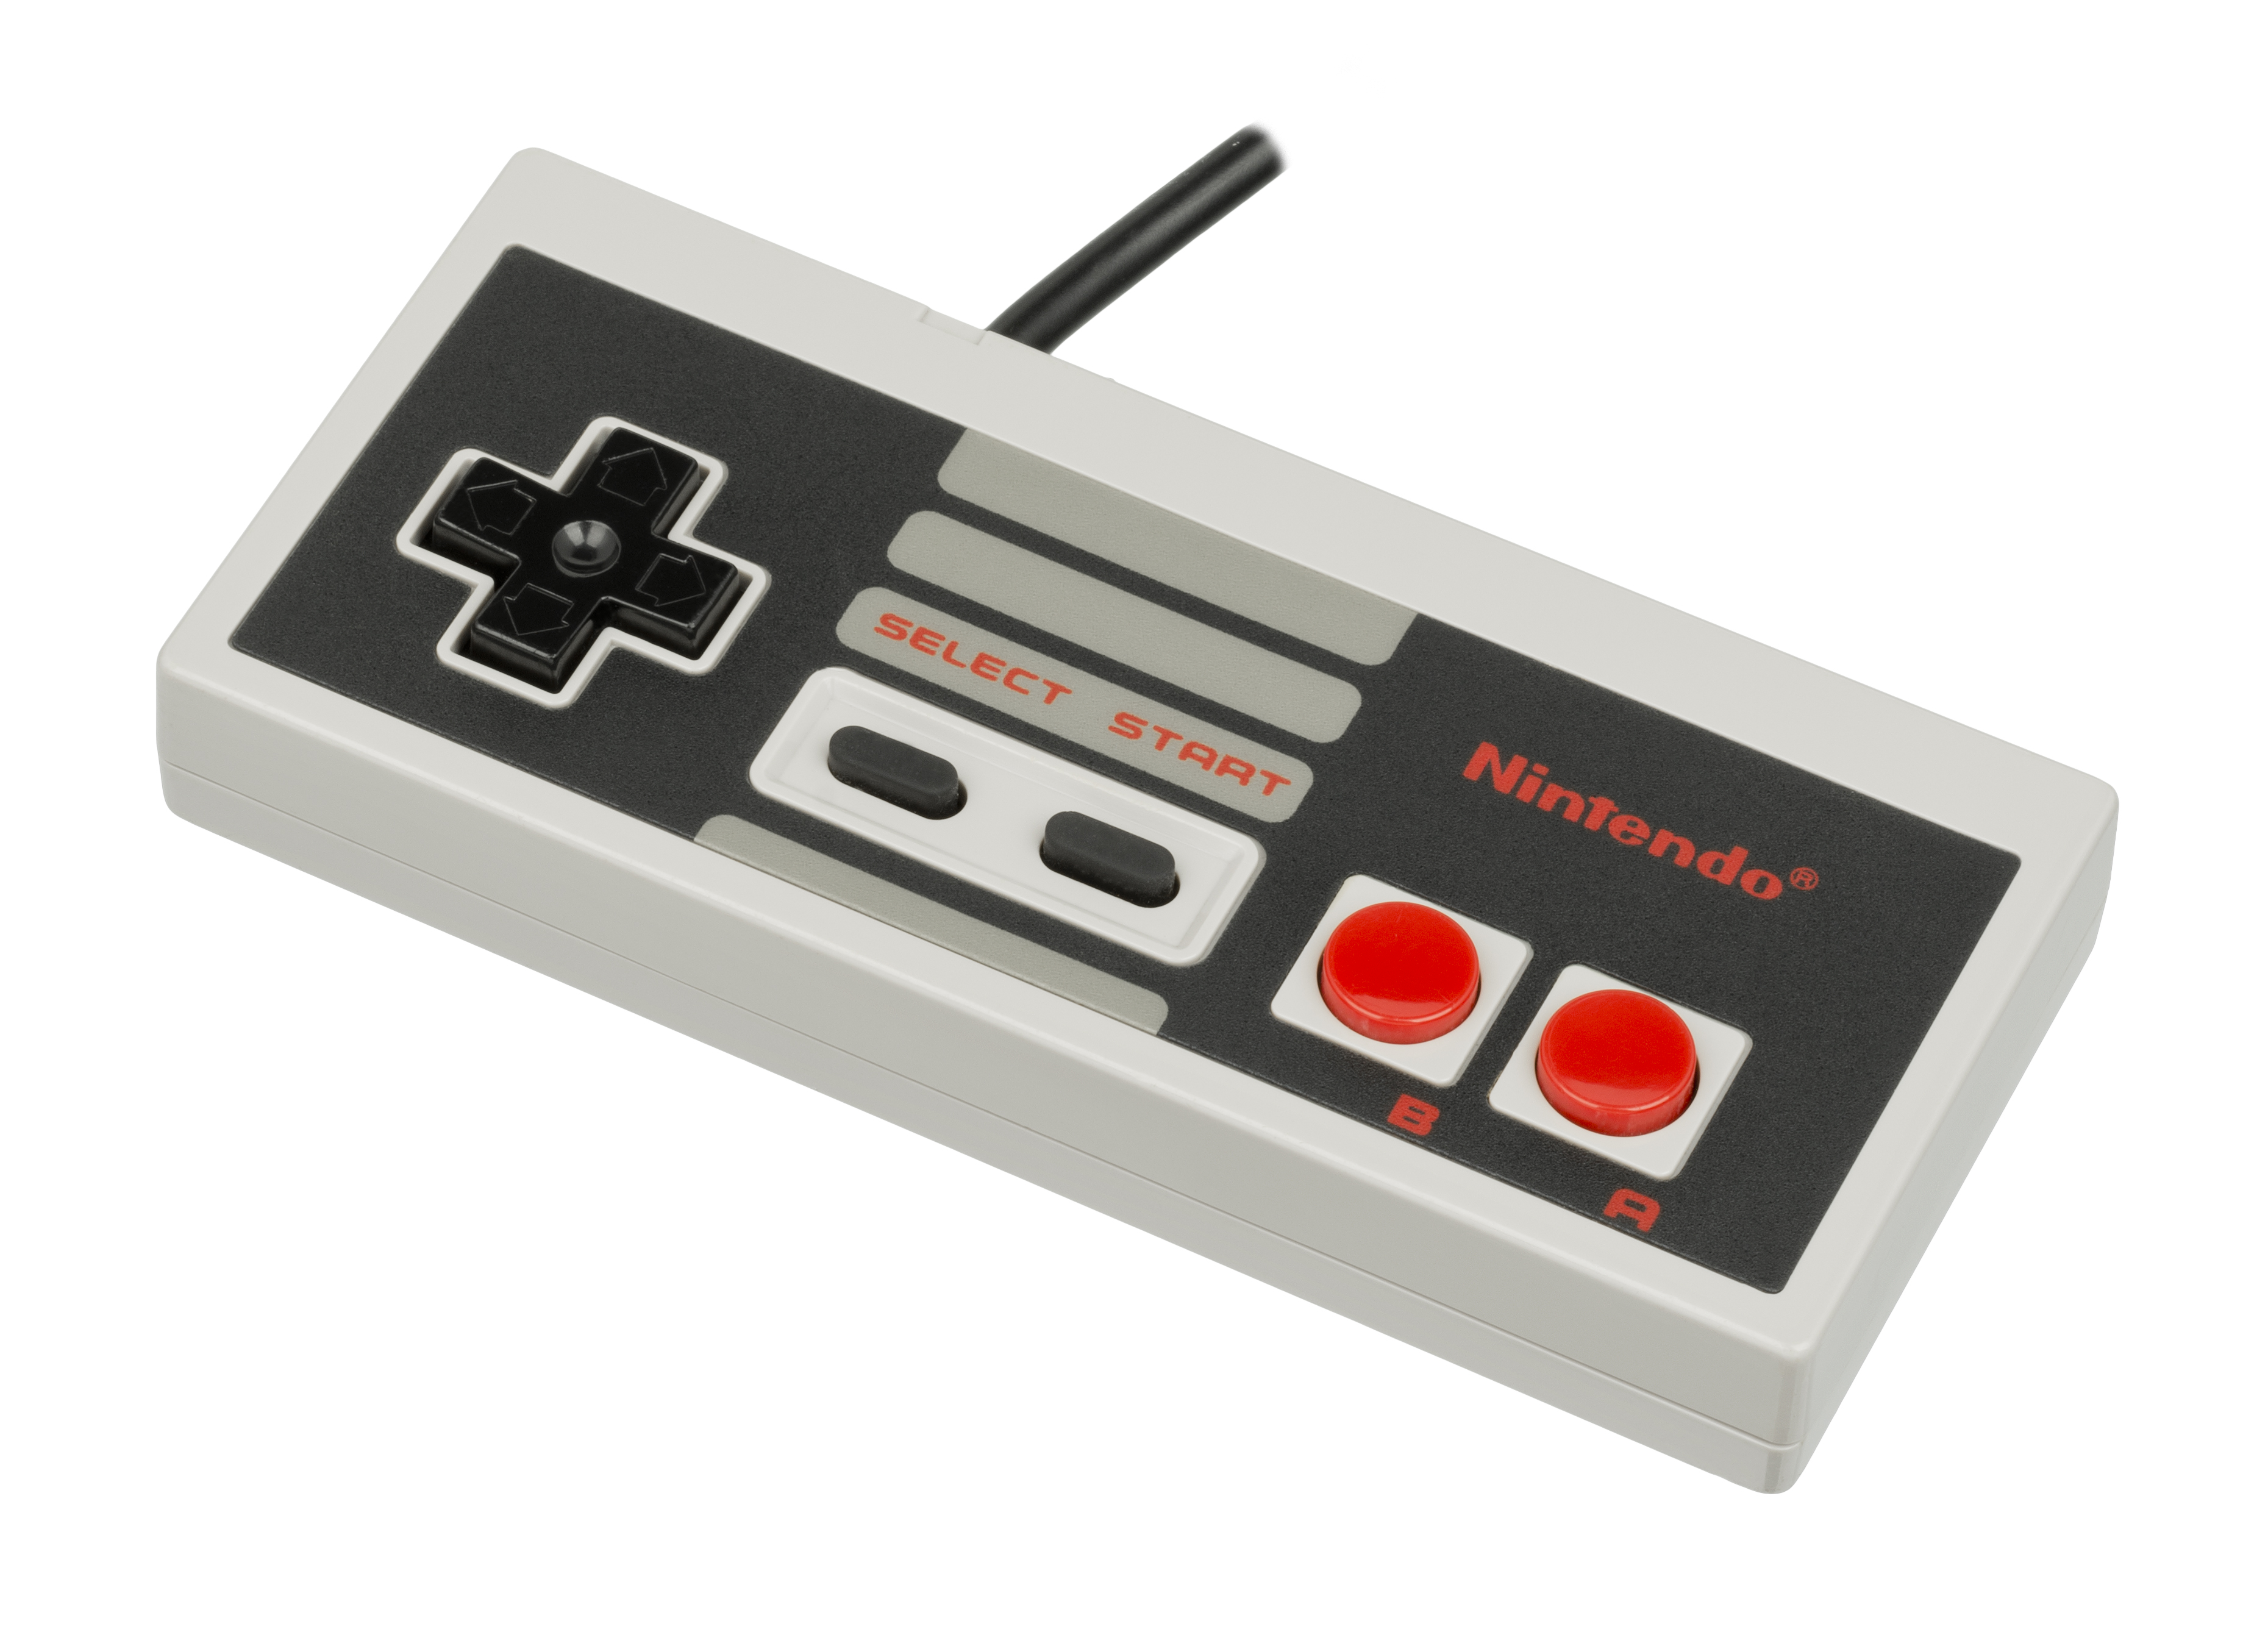
\includegraphics[width=0.5\textwidth]{images/nes-ovladac.jpg}
\end{figure}

Periferie jsou mapovány do paměti; čtení i~zápis tedy probíhají stejným způsobem, jako do každého jiného registru. První ovladač je mapován na adresu \$4016, druhý na sousední \$4017.

Při čtení jsou k~dispozici všechny tři piny, které jsou umístěny do jednotlivých bitů dle svého označení, tedy D0 na nejnižším bitu a tak dále. Tabulka~\ref{tab:periferie-cteci-piny} ukazuje, jakou mají piny funkci.

\begin{table}[ht!]
	\centering
	\caption{Funkce vstupních pinů portů konzole}\label{tab:periferie-cteci-piny}
	\begin{tblr}{|Q[c,m]|Q[c,m]|}
		\hline
		Pin & Funkce \\
		\hline[2pt]
		D0 & Sériový výstup stavů tlačítek ovladače \\
		\hline
		D3 & Výstup světelného senzoru periferie Zapper \\
		\hline
		D4 & Stav spouště periferie Zapper \\ 
		\hline
	\end{tblr}
\end{table}

Stav tlačítek se vyčítá z~jediného bitu: D0. Jedná se o~sériový výstup osmibitového paralelně-sériového posuvného registru a~to, co je na jeho výstupu, záleží na stavu ovládacího klopného obvodu, který je k~dispozici pouze na nejnižším bitu adresy \$4016 (\$4017 je pouze pro čtení). Logickou jedničkou se aktivuje obnova stavu tlačítek do vnitřních registrů a~na výstupu je neustále stav jediného tlačítka (A). Přivedením nuly je pak možné postupně vyčíst hodnotu stisknutých tlačítek v~následujícím pořadí: A, B, Select, Start, Up, Down, Left, Right. Jelikož stisk tlačítka přivede na výstup logickou nulu, dochází k~dodatečné inverzi hodnoty tak, aby stisknuté tlačítko vracelo logickou jedničku a~puštěné logickou nulu~\cite{Nesdev:standard-controller}.

Po přečtení tlačítek vrací výstup logickou jedničku. To je způsobeno tím, že na sériový vstup posuvného registru (který se používá pro řetězení více takových posuvných registrů) je přivedeno nízké napětí (logická nula), což po dodatečné inverzi odpovídá logické jedničce. Pro další čtení je nutné opět obnovit stavy tlačítek~\cite{Nesdev:standard-controller}.

Standardní postup při čtení by se tedy dal shrnout takto:
\begin{enumerate}
	\item Zapsání logické jedničky do bitu 0 na adrese \$4016.
	\item Zapsání logické nuly do stejného místa.
	\item Postupné vyčítání osmi bitů ze sériového portu na adrese dle požadovaného ovladače (\$4016 či \$4017).
\end{enumerate}

\section{Audio Processing Unit}
\label{sec:APU}
Součástí procesoru Ricoh~2A03 je také zvukový syntezátor, přezdívaný jako Audio Processing Unit (APU).

\section{Existující řešení}


%---------------------------------------------------------------
\chapter{Návrh}
%---------------------------------------------------------------
\epigraph{
	\enquote{Simplicity is prerequisite for reliability.}
}{\textsc{Edsger W. Dijkstra}}

\section{Úvod}
Při analýze byly získány potřebné informace o~tom, z~čeho se NES skládá a~jak tyto komponenty fungují. Po analyzování systému je třeba navrhnout, jak jej prakticky implementovat. Vzhledem k~tomu, že je cílem projektu být co nejsrozumitelnější, je nutné brát v~potaz nejen návrh implementace samotného systému, ale i~emulační platformy, na které emulovaný systém poběží.

Nejprve je třeba navrhnout technologie, které se pro implementaci využijí. Dále je nutné navrhnout univerzální rozšiřitelnou platformu. Nakonec se za pomocí určených technologií a~platformy navrhne, jak implementovat samotnou konzoli NES.

\section{Výběr technologií}
Na začátku vývoje je třeba vybrat správné nástroje tak, aby byl vývoj co nejefektivnější a~nejpohodlnější. Kromě jmenovaných požadavků je nutné brát v potaz také externí požadavky, které stanovuje jednak zadání, jednak výsledky samotného bádání v~analytické části.

\subsection{Programovací jazyk}
Zadání požaduje, aby byl emulátor implementován s~využitím principů OOP, které byly popsány v~části \ref{sec:OOP}. Vhodnost k~využití ve výuce pak znamená, že je třeba využít rozšířený jazyk, nebo takový jazyk, jehož syntaxe je běžným jazykům podobná. Nepřímo také vyplývá, že by mělo být možné výsledný kód spouštět na co největším množství platforem tak, aby byl emulátor, jakožto vzdělávací pomůcka, snadno dostupný. Nakonec se při výběru je nutné zaměřit na to, že se jedná o~implementaci počítačového systému. Zvolený jazyk by tedy neměl poskytovat příliš velkou abstrakci nad počítačovým hardwarem --- to by mohlo způsobit odstínění od vysvětlovaných principů.

Zvoleným jazykem pro implementaci je C++ ve verzi C++20. Splňuje totiž veškeré požadavky dané zadáním i~ze zadání vyplývajících:
\begin{itemize}
	\item podpora paradigmatu OOP,
	\item náklonnost k systémovému programování,
	\item umožňuje výběr míry abstrakce programátorem,
	\item podpora mnoha platforem,
	\item syntaxe podobná jiným rozšířeným C-like jazykům.
\end{itemize}

\subsection{Kolekce vývojových nástrojů}
\begin{definition}[Toolchain]
	Toolchain je anglický termín pro kolekci nástrojů využívaných při vývoji. Typicky se jedná o~soubor prostředí pro vývoj: textový editor pro psaní zdrojového kódu, kompilátor pro překlad do strojového kódu, linter pro kontrolu syntaktických chyb (dnes existují nástroje i~pro hledání různých sémantických chyb, například nástroj clang-tidy), debugger.
\end{definition}

\subsection{Správa zdrojového kódu}

\subsection{Dokumentace}

\subsection{Testování}
Aby byl zajištěn soulad s~požadavky, je nutné program testovat. Úkolem této části je stanovit požadavky na testy a~na tom základu navrhnout vhodné metodiky a~nástroje.

Ačkoliv je možné testování provést až na konci, je vhodné \emph{testovat průběžně}, aby bylo možné chyby diagnostikovat \emph{izolovaně}. Mohlo by totiž dojít k~situaci, kdy se chyba v~jedné komponentě projeví v~jiné, což přináší velmi těžce diagnostikovatelné problémy. Není však reálné provádět průběžné testy ručně, cílem tedy je navrhnout \emph{automatické testy}.

Spouštění testů v~základní formě vyžaduje akci programátora, což přináší riziko lidského faktoru v~podobě zapomenutí, především u~jednoduchých změn. Existují však nástroje, které umí i~spouštění testů provádět automaticky. Je rozumné se zaměřit především na \emph{testování před přijetím změn} --- nedovolit sloučit změny do hlavní vývojové větve v~repozitáři před tím, než se otestuje, zdali změny nevnesly nové chyby.

Specifikem bakalářské práce je fakt, že implementuje emulaci systému, od které se očekává, že bude věrně napodobovat emulovaný systém. Dalším požadavkem je proto možnost \emph{spouštět testy ve formě strojového kódu} pro danou platformu s~možností automatického vyhodnocení. Pro archaické systémy vzniklo již mnoho testů, které mají za úkol porovnat funkci s~reálným systémem. Sofistikované testy umožňují vybrat druh výstupu, kdy součástí bývá i~zápis výsledků do vybraného místa v~paměti.

Jak bylo uvedeno v~kapitole \ref{sec:teorie-testovani}, testy se dají provádět ručně i~automaticky. Jelikož je požadováno průběžné testování, je nejvhodnější co nejvíce testů automatizovat. To vyžaduje nástroj pro spouštění a~řízení testů. Součástí nástroje CMake je CTest, který je využit i~v~této práci.

Pro samotné psaní testů již není třeba další komponenty, 

\section{Emulační platforma}

%---------------------------------------------------------------
\chapter{Implementace}
%---------------------------------------------------------------
\epigraph{
	\enquote{If you love what you do and are willing to do what it takes, it's within your reach.}
}{\textsc{Steve Wozniak}}

%---------------------------------------------------------------
\chapter{Testování}
%---------------------------------------------------------------

\section{Testování procesoru 6502}
\subsection{Příprava testů}
Emulovaný procesor 6502 byl testován existujícími testy. Základní implementace byla testována pomocí sady testů od Klause Dormanna. Testy jsou ve formě JSA, kde je možné nakonfigurovat základní parametry testu. Tento test používá pro vyhodnocování výsledků pasti (viz sekce~\ref{sec:testovaci-programy}), tedy zacyklení v~případě dokončení testu (úspěšného i~neúspěšného).

Jelikož byl v~návrhu stanoven požadavek automatizace testů, je nutné vytvořit pipeline, která testy sestaví a~publikuje tak, aby je bylo možné stáhnout a~spustit zcela bez zásahu člověka.

Pro účely vývoje emulátoru byl vytvořen fork originálního repozitáře s kódy na adrese \url{https://github.com/andreondra/use-tests-6502-65C02}. V~tomto repozitáři byly testy nakonfigurovány dle potřeb a~vytvořen skript pro automatické sestavování nástrojem GitHub Actions.

Test pro ověření funkce přerušení vyžaduje mapování pinů NMI a IRQ do paměti tak, aby je bylo možné ovládat programově. Součástí nastavení je tedy adresa mapování, způsob řízení a umístění signálů dle bitů. Ve výpisu~\ref{list:6502-test-konfigurace} jsou čtyři konfigurované položky.

\begin{listing}
	\caption{Příklad konfigurace testu pro procesor 6502}
	\label{list:6502-test-konfigurace}
	\begin{minted}{ca65}
I_port    = $bffc   ; Adresa mapovani do pameti.
I_drive   = 0       ; 0 = prime rizeni, 1 = otevreny kolektor.
IRQ_bit   = 0       ; Cislo bitu prirazene IRQ.
NMI_bit   = 1       ; Cislo bitu prirazene NMI (-1, neni-li k dispozici).
	\end{minted}
\end{listing}

Po patřičném nastavení testů je možné vytvořit konfiguraci automatického sestavení. Přímo v~repozitáři je vytvořen soubor \mintinline{text}|build-release.yaml| v~adresáři \mintinline{text}|.github/workflows|. Tato konfigurace při každé změně spustí virtuální stroj, zkompiluje zdrojové kódy a~publikuje je v~novém vydání. Samotná kompilace probíhá pomocí assembleru as65, který je obsažen přímo v~repozitáři (na původní webové stránce již není k~dispozici). Výpis~\ref{list:6502-test-sestaveni} ukazuje výňatek, ve kterém je spouštěn kompilátor i~s~popisem použitých přepínačů. Velice důležitý je přepínač \mintinline{text}|-l|, který vygeneruje listing (viz kapitola~\ref{sec:teorie-testovani}). Pomocí něj je možné určit, v~jaké části programu došlo zacyklení, a~tedy jestli byl test úspěšný či nikoliv a~proč.

\begin{listing}
	\caption{Kompilace testů v automatickém sestavení}
	\label{list:6502-test-sestaveni}
	\begin{minted}{yaml}
jobs:
    build-and-release:
        runs-on: ubuntu-latest
        steps:
          # ...
          # Pouzite prepinace:
          # -lw = vygeneruje se siroky listing
          # -m  = vypisi se makra
          # -t  = vygeneruje se tabulka symbolu
          - name: Assemble the sources
            run: |
              as65/as65 -l -mwt 6502_functional_test.a65
              as65/as65 -l -mwt 6502_decimal_test.a65
              as65/as65 -l -mwt 6502_interrupt_test.a65
	\end{minted}
\end{listing}

Výsledkem každé změny je soubor spustitelných programů ve formě strojového kódu a~odpovídající výpisy, jak ukazuje obrázek~\ref{fig:vydani-testu-6502}.

\begin{figure}[ht!]
	\centering
	\caption{Vydání testů pro procesor 6502}
	\label{fig:vydani-testu-6502}
    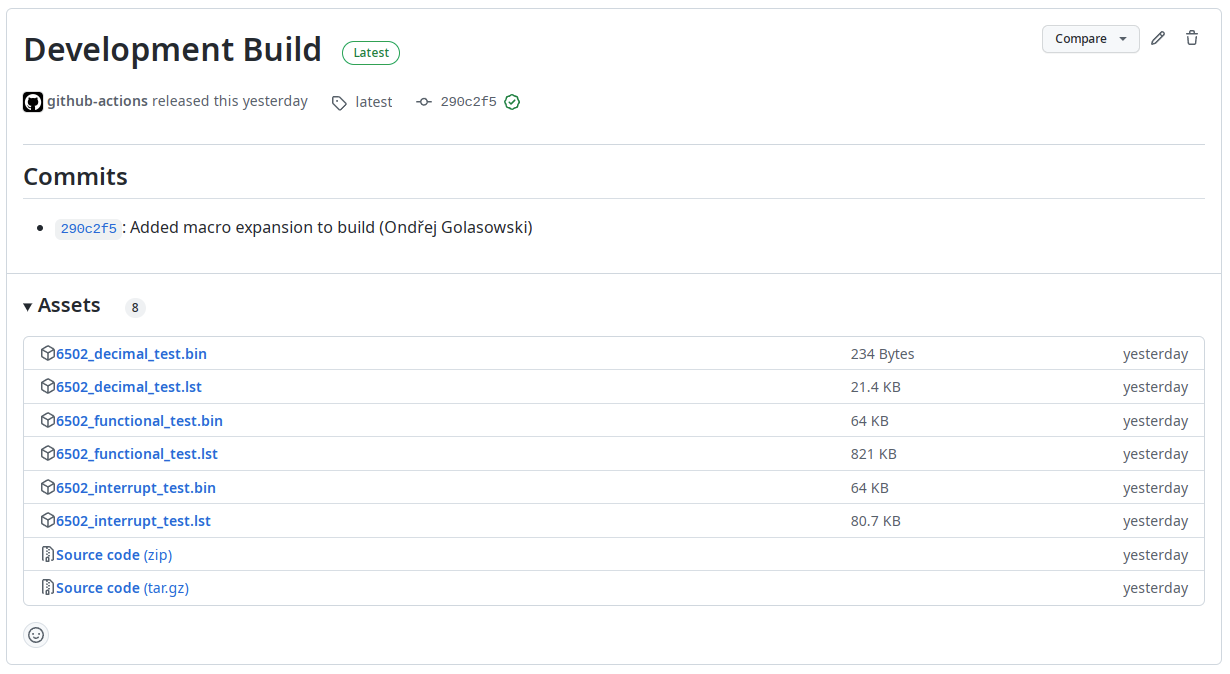
\includegraphics[width=0.8\textwidth]{images/vydani-testu-6502.png}
\end{figure}

\subsection{Integrace s Google Test}
Nakonfigurované a sestavené testy je nyní možné spouštět ručně. Pro automatické spouštění je nutné vytvořit testovací funkci pro platformu Google Test. Aby byly dodržovány zásady dobrého testování, je vhodné test vytvořit za použití existující komponenty, do které se nebudou přidávat žádné funkcionality pouze pro běh testu. Případné změny lze totiž provést přímo v~testu, a~to za použití dědičnosti. Ve výpisu~\ref{list:6502-test-uprava} je znázorněna upravená třída procesoru. Je použit název DUT (design under test), který se používá například při tvorbě testů ve VHDL. Důležitou úpravou je přidání rozhraní pro úpravu programového čítače, což je nutné pro spuštění testu a~kontroly stavu testu.

\begin{listing}
	\caption{Upravený procesor 6502 v Google Test}
	\label{list:6502-test-uprava}
	\begin{minted}{c++}
    class DUT : public MOS6502 {
	public:
	void step() {
		while(!instrFinished()) {
			CLK();
		}
		CLK();
	}
	uint16_t getPC() {
		return m_registers.pc;
	}
	void setPC(uint16_t val) {
		m_registers.pc = val;
	}
	void triggerNMI() {
		NMI();
	}
	void setIRQ(bool active) {
		IRQ(active);
	}
};
	\end{minted}
\end{listing}

Samotný test pak probíhá v~jednoduchém cyklu, kde podmínkou pro opuštění je opakovaná hodnota programového čítače. Ověření výsledku probíhá porovnáním poslední hodnoty programového čítače. Dle listingu vygenerovaného assemblerem lze zjistit, že úspěch je signalizován zacyklením na adrese \mintinline{text}|$06e5|, což ukazuje výňatek ve výpisu~\ref{fig:6502-test-uspech}. Celý testovací cyklus s~ověřením výsledku se nachází ve výpisu~\ref{list:6502-test-cyklus}.

\begin{listing}
	\caption{Řádek signalizující úspěch v listingu testu 6502}
	\label{fig:6502-test-uspech}
	\begin{minted}{ca65}
                                success         ; Navesti makra uspechu.
06e5 : 4ce506          >        jmp *           ; Test byl dokoncen uspesne.
	\end{minted}
\end{listing}

\begin{listing}
	\caption{Testovací cyklus procesoru 6502 v Google Test}
	\label{list:6502-test-cyklus}
	\begin{minted}{c++}
do {
	prevPC = cpu.getPC();
	cpu.step();
} while(prevPC != cpu.getPC());

EXPECT_EQ(prevPC, ADR_SUCCESS) 
	<< "The test failed on trap at address 0x"
	<< std::hex << prevPC;
	\end{minted}
\end{listing}


\subsection{Příklad testování}
Jedním z~problému, které se v~průběhu vývoje objevily, byl problém s~časováním přerušení. Byla proto vytvořena verze, která lépe odpovídá skutečnému chování. Kvůli tomu ale přestal fungovat test přerušení: \mintinline{text}|6502_interrupt_test.bin|. Tato část popisuje, jak se dá podobná chyba diagnostikovat a~opravit.

Test se zastavil na adrese \mintinline{text}|$6b2|. Dle listingu tato adresa odpovídá sekci, kde se testují oba přerušení, NMI a~IRQ. Část způsobující chybu je vyobrazena ve výpisu~\ref{list:6502-test-hledani-chyby}. Nejprve se nastaví vyvolání obou typů přerušení instrukcí \mintinline{text}|sta I_port|, přičemž IRQ bylo maskováno (pro stručnost není proces maskování uveden). Čeká se na provedení obslužné rutiny NMI a~otestuje se, zdali proběhlo. Poté se povolí přerušení IRQ instrukcí \mintinline{text}|cli|. Nyní by měla proběhnout rutina IRQ, k~tomu však nedojde a~test se zastaví.

\begin{listing}
	\caption{Příklad konfigurace testu pro procesor 6502}
	\label{list:6502-test-hledani-chyby}
	\begin{minted}{ca65}
; Testovani IRQ a NMI s maskovanim preruseni.
; ...
												; Testovani NMI
0699 : 8dfcbf          >        sta I_port      ; Vyvolani preruseni.

069c : e8                       inx
069d : e8                       inx
069e : e8                       inx
069f : ad0302                   lda I_src       ; Probehlo preruseni?
                                trap_ne
06a2 : d0fe            >        bne *           ; Pokud ne, skonci test.

06a4 : a200                     ldx #0

06a6 : a902                     lda #2          ; Testovani IRQ
06a8 : 8d0302                   sta I_src
06ab : 58                       cli             ; Povoleni IRQ.
06ac : e8                       inx
06ad : e8                       inx
06ae : e8                       inx
06af : ad0302                   lda I_src       ; Probehlo preruseni?
                                trap_ne
06b2 : d0fe            >        bne *           ; Pokud ne, skonci test.
	\end{minted}
\end{listing}

Již na základě této množiny informací lze chybu nalézt. Test nastaví zpětnovazební registr tak, aby byla vyvolána oba přerušení již při prvním testu, kdy se ověřuje NMI. V~dalším testu (ověření IRQ) již pouze povolí přerušení a~hodnotu ve zpětnovazebním registru nemění.

Skutečný procesor 6502 každé přerušení detekuje jiným způsobem. Přerušení IRQ detekuje úrovňový detektor. Při logické nule se zaznamená požadavek na přerušení a~po dokončení stávající instrukce se ověří, zdali přerušení není maskováno. Pokud je, provede se další instrukce normálním způsobem a~požadavek se zahodí. Tento požadavek je ale znovu zaznamenán, pokud je signál stále aktivní (tedy na logické nule). Emulovaný procesor vyvolal při zápisu do zpětnovazebního registru pouze jeden požadavek, choval se tedy jako hranový detektor, což je v~rozporu se skutečným procesorem, a~proto toto chování test vyhodnotil jako chybné. Hranový detektor je použit pouze u~NMI.

Stačí tedy funkci odpovídající pinu IRQ implementovat tak, aby se dal nastavovat jeho stav (aktivní a neaktivní), nikoliv pouze vyvolávat signál, jako je to u~NMI. Klíčovou část kódu ukazuje výpis~\ref{list:6502-preruseni-irq-oprava}.

\begin{listing}
	\caption{Oprava chybné implementace IRQ}
	\label{list:6502-preruseni-irq-oprava}
	\begin{minted}{c++}
void MOS6502::IRQ(bool active){
	m_irq = active;
}
	\end{minted}
\end{listing}


\begin{note}[Funkčnost původní implementace]
A proč tedy původní implementace fungovala? To bylo způsobeno jinou chybou, kdy se požadavek na přerušení ukládal, pokud bylo přerušení maskováno. To ale také neodpovídá skutečnému procesoru.
\end{note}

\subsection{Další testy}
TODO Popsat nestest a další.
 % include `text.tex' from `text/' subdirectory

\appendix\appendixinit % do not remove these two commands

\chapter{Nějaká příloha}


Sem přijde to, co nepatří do hlavní části.

\begin{figure}[p!]
	\centering
	\caption{Přehledové hardwarové schéma konzole NES. Obrázek \enquote{NES-001 Console} vytvořil schenkzoola pod licencí CC~BY~4.0.}
	\label{fig:nes001-hw}
	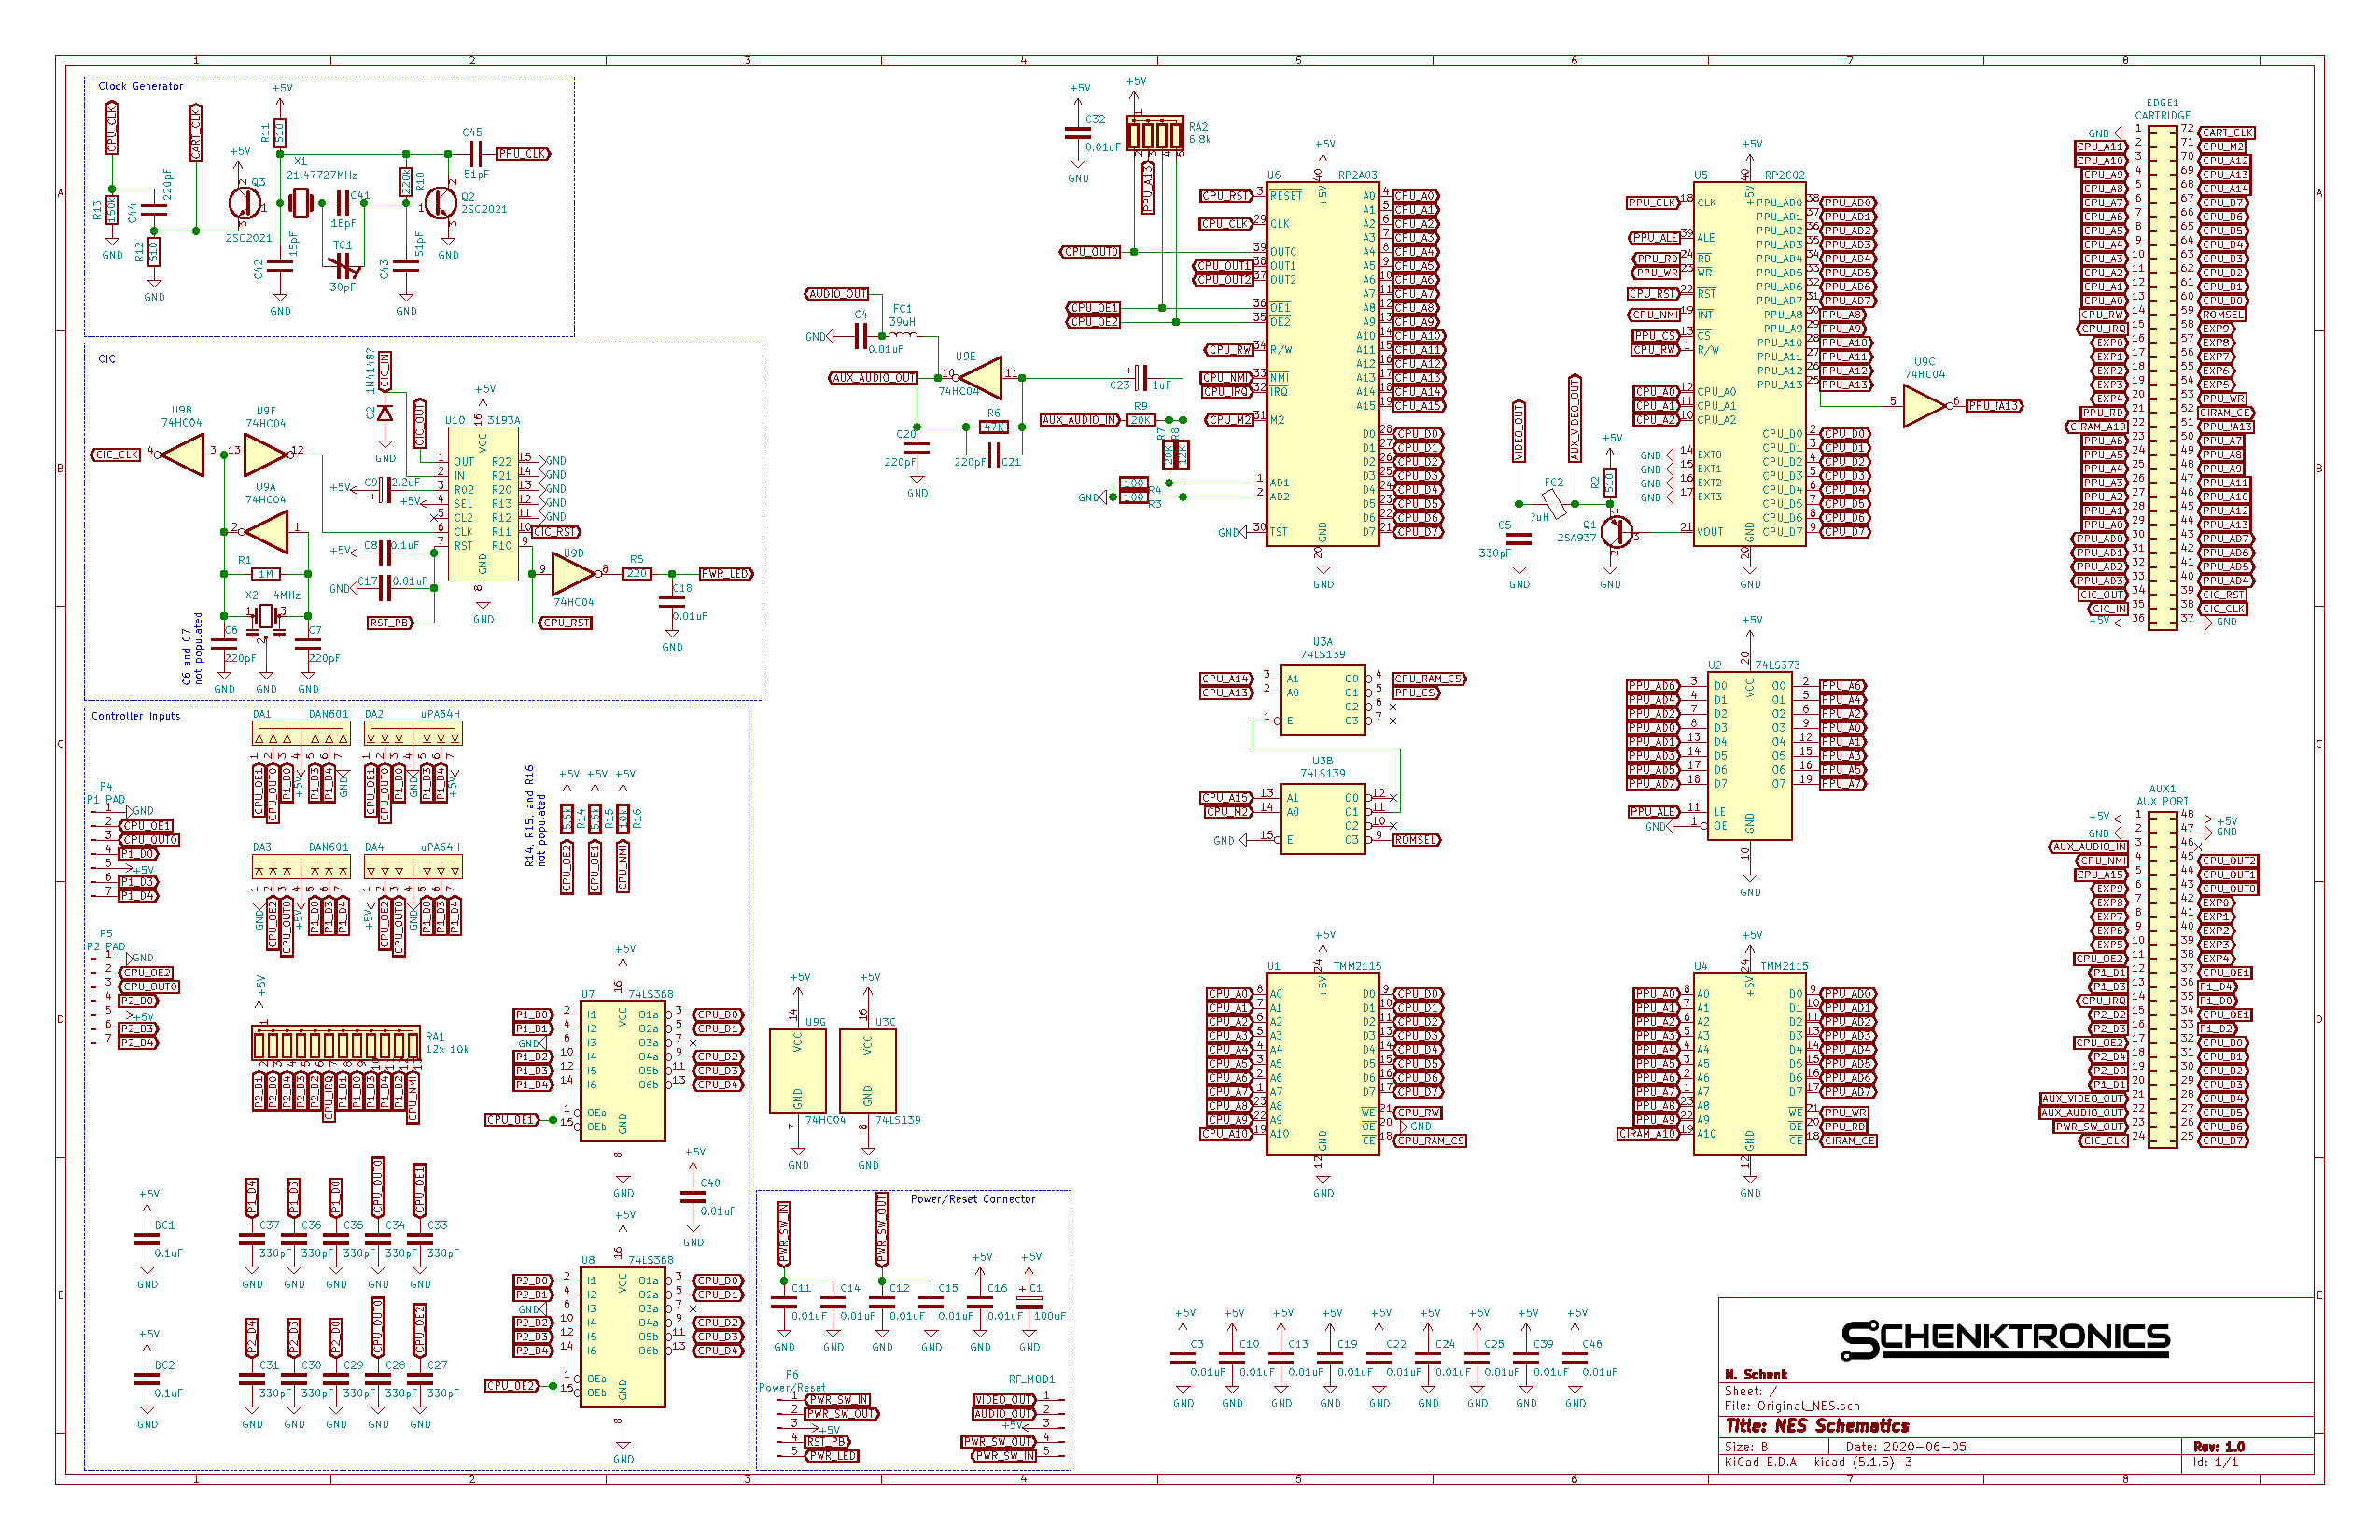
\includegraphics[width=0.95\textheight, angle=270]{images/NES-001.pdf}
\end{figure}

\chapter{Knihovna ImInputBinder}
\label{apx:binder}

Knihovna ImInputBinder vznikla jako rozšíření pro projekt Universal System Emulator. % include `appendix.tex' from `text/' subdirectory

\backmatter % do not remove this command

\printbibliography % print out the BibLaTeX-generated bibliography list

\chapter{Obsah přiloženého média}


	\dirtree{%
		.1 readme.txt\DTcomment{stručný popis obsahu média}.
		.1 exe\DTcomment{adresář se spustitelnou formou implementace}.
		.1 src.
		.2 impl\DTcomment{zdrojové kódy implementace}.
		.2 thesis\DTcomment{zdrojová forma práce ve formátu \LaTeX{}}.
		.1 text\DTcomment{text práce}.
		.2 thesis.pdf\DTcomment{text práce ve formátu PDF}.
	}
 % include `medium.tex' from `text/' subdirectory

\end{document}
